\NeedsTeXFormat{LaTeX2e}
\documentclass[
    a4paper,
    10pt,
    bibliography=totoc,
    twoside,
    openright,
    numbers=noenddot,
    headings=normal,
    DIV=9,
    BCOR=7mm
    ,parskip
]{scrbook}

\usepackage[utf8]{inputenc}
\usepackage[UKenglish]{babel}
\usepackage[babel]{csquotes}

\usepackage{lmodern}
%\usepackage{times}
%\usepackage{helvet}
\usepackage[T1]{fontenc}


%%
%% Schriftarten
%%
\renewcommand{\sfdefault}{phv}
\renewcommand{\rmdefault}{phv}
\renewcommand{\ttdefault}{pcr}
%\KOMAoptions{DIV=last}



%%
%% Diverse Pakete
%%
\usepackage{ccicons} % Creative Commons Lizenzsymbole
\usepackage{enumitem} % Àndern von listeneinstellungen mit \setlist
\setlist{nolistsep} % kein abstand zwischen items in listen, Befehl von enumitem
\usepackage{float} % use \begin{figure}{H} to really force a figure being placed here
\usepackage[section]{placeins} % floatbarrier at each new section, so every figure appears in its own section


\usepackage{scrhack}
\usepackage{graphicx}
\usepackage{verbatim}
\usepackage{tabularx}
\usepackage{url}
\usepackage{xcolor}
\usepackage{amssymb}
\usepackage{amsmath}
\usepackage{amsthm}
\usepackage{setspace}
\usepackage{listings}
\usepackage{colortbl}
%\usepackage{showframe} % Seitenspiegel anzeigen

\usepackage[activate={true,nocompatibility},final,tracking=true,kerning=true,spacing=true,factor=1100,stretch=10,shrink=10]{microtype}

\usepackage{hyperref} 

\hyphenation{so-phis-ti-cat-ed con-fig-u-ra-tion}


\usepackage[euler]{textgreek}

\usepackage{csvsimple}
\usepackage{longtable}
\usepackage{booktabs}
\usepackage{rotating}

\usepackage{graphicx}
\usepackage{caption}
\usepackage{subcaption}

\usepackage{import}

\usepackage{tabularx}

\usepackage[nohyperlinks,printonlyused]{acronym}

\usepackage{wasysym}

\usepackage{pgfplots}
\usepackage{tkz-base}

\usepackage{wrapfig}
\usepackage{boxhandler}

\usepackage{siunitx}
\usepackage{xfrac}

\usepackage{xcolor}

\newsavebox\IBoxA \newsavebox\IBoxB \newlength\IHeight
\newcommand\TwoFig[8]{% Image1 Caption1 Label1 Image2 ...
  \sbox\IBoxA{\includegraphics[width=0.45\textwidth]{#1}}
  \sbox\IBoxB{\includegraphics[width=0.45\textwidth]{#4}}%
  \ifdim\ht\IBoxA>\ht\IBoxB
    \setlength\IHeight{\ht\IBoxB}\else\setlength\IHeight{\ht\IBoxA}\fi%
  \begin{figure}[!htb]
  \begin{subfigure}[b]{0.45\textwidth}
  \centering
  \includegraphics[height=\IHeight]{#1}
  \caption{#2}\label{#3}
  \end{subfigure}
  \hfill
  \begin{subfigure}[b]{0.45\textwidth}
  \centering
  \includegraphics[height=\IHeight]{#4}
  \caption{#5}\label{#6}
  \end{subfigure}
  \caption{#7}\label{#8}
  \end{figure}%
}

\usepackage[]{todonotes} %[disable]

\usepackage[
style=alphabetic,    % Zitierstil
isbn=false,                % ISBN nicht anzeigen, gleiches geht mit nahezu allen anderen Feldern
url=true,
pagetracker=true,          % ebd. bei wiederholten Angaben (false=ausgeschaltet, page=Seite, spread=Doppelseite, true=automatisch)
maxbibnames=50,            % maximale Namen, die im Literaturverzeichnis angezeigt werden (ich wollte alle)
maxcitenames=2,            % maximale Namen, die im Text angezeigt werden, ab 4 wird u.a. nach den ersten Autor angezeigt
autocite=inline,           % regelt Aussehen fÃŒr \autocite (inline=\parancite)
block=space,               % kleiner horizontaler Platz zwischen den Feldern
backref=false,              % Seiten anzeigen, auf denen die Referenz vorkommt
%backrefstyle=three+,       % fasst Seiten zusammen, z.B. S. 2f, 6ff, 7-10
date=short,                % Datumsformat
backend=bibtex,
hyperref=true
]{biblatex}
\setlength{\bibitemsep}{1em}     % Abstand zwischen den Literaturangaben
\setlength{\bibhang}{2em}        % Einzug nach jeweils erster Zeile

\bibliography{bibliography}  % Bibtex-Datei wird schon in der Preambel eingebunden

\newcommand{\fullname}{Pascal Knierim}
\newcommand{\email}{pascal.knierim@uni-ulm.de}
\newcommand{\titel}{A Novel Projector Camera System for Effortless Domestic Deployment}
\newcommand{\jahr}{2014}
\newcommand{\matnr}{651625}
\newcommand{\gutachterA}{Prof.\ Dr.\ Enrico Rukzio}
\newcommand{\gutachterB}{Prof.\ Dr.\ Michael Weber} % -Ing. ????
\newcommand{\betreuer}{Prof.\ Dr.\ Enrico Rukzio} 
\newcommand{\fakultaet}{Engineering\\and Computer Science}
\newcommand{\institut}{Institute of Media Informatics}
\newcommand{\arbeit}{Master Thesis}

\newtheorem{definition}{Definition}[chapter]
\newtheorem{example}{Example}[chapter]

\pdfinfo{
    /Author (\fullname)
    /Title (\titel)
    /Producer (pdfTeX, Version 3.1415926-2.5-1.40.14)
    /Keywords ()
}
\hypersetup{
    pdftitle=\titel,
    pdfauthor=\fullname,
    pdfsubject={\arbeit},
    pdfproducer={pdfTeX, Version 3.1415926-2.5-1.40.14},
    colorlinks=false,
    pdfborder=0 0 0
}

\setcounter{tocdepth}{2}

\clubpenalty10000
\widowpenalty10000
\displaywidowpenalty=10000

\definecolor{Uulmin}{RGB}{163,38,56} 

\lstset{
    language=Prolog,
    showstringspaces=false,
    frame=single,%L,%TB,%single
    breaklines=true,
    breakatwhitespace=true,
    numbers=left,
    aboveskip=\parskip,
    basicstyle=\ttfamily,
    numberstyle=\tiny,
    deletekeywords={ time, is, name, write, true, false, fail, or, length },
    keywordstyle=\bfseries,
    alsoletter= {<,=,>,:,-,@, |, \\, ? },
    morekeywords={ <=>, ==> , :-, @, |, \\, ?- },
    morecomment=[s]{\{}{\}},
    moredelim=[is][\textbf]{<<}{>>},
    moredelim=[is][\textit]{<<<}{>>>}
}

\newcommand{\FIXME}[1]{} % deploy mode

% multi-letter variables in math mode
\newcommand*{\var}[1]{\mathord{\mathit{#1}}}
% relations in math mode
\newcommand*{\rel}[1]{\mathord{\mathrm{#1}}}
% functions in math mode
\newcommand*{\fun}[1]{\mathord{\mathit{#1}}}

\setlength{\arrayrulewidth}{0.1pt}

\pagestyle{headings}

\renewcommand{\labelitemi}{$\bullet$}
\renewcommand{\labelitemii}{$\circ$}
\renewcommand{\labelitemiii}{$\cdot$}

\begin{document}

\frontmatter

\thispagestyle{empty}

\begin{addmargin*}[4mm]{-32mm}
    
\includegraphics[height=1.8cm]{images/uni_logo/uni_bild}
    \hfill
    
\includegraphics[height=1.8cm]{images/uni_logo/uni_wort}
    \vspace*{2.1em}
    \footnotesize
    {\fontfamily{phv}\selectfont
    
    \textbf{Ulm University} \textbar ~89069 Ulm \textbar ~Germany
    \hfill
    \parbox[t]{42mm}{\bfseries Faculty of \fakultaet\\\mdseries\institut}
    \vspace*{2cm}

    \parbox{140mm}{\bfseries \raggedright \huge A Novel Projector Camera System\\ for Effortless Domestic Deployment}

    {\arbeit{}\\Ulm University}
    \vspace*{4em}

    \fullname\\\email\\[2em]
    \textbf{Reviewers:}\\\gutachterA\\\gutachterB\\[2em]
    \textbf{Consultant:}\\\betreuer\\[1.5em]
    \jahr}
\end{addmargin*}


\clearpage
\thispagestyle{empty}
{
    \small \flushleft \enquote{\titel}\\
    \today
    \vfill

    \copyright{} \jahr{} \fullname{}\\[0.5em]
    This work is licensed under a Creative Commons Attribution-ShareAlike 3.0 License: \url{http://creativecommons.org/licenses/by-sa/3.0/}\\
    \ccbysa\\
    \vspace{0.5cm}
    Typesetting: PDF-\LaTeXe{}\\
    Graphics created with: Ti\textit{k}Z\\
    Printed by: Kommunikations- und Informationszentrum (kiz), University of Ulm
}

\setstretch{1.2} 
\renewcommand{\arraystretch}{1.2} 

% !TEX root = ../arbeit.tex
\chapter*{Abstract}
Providing instant access to information when and wherever it is desired is one of the aims of the ubiquitous computing research area. To accomplish omnipresent visualisation of information, display technology needs to be present everywhere. As modern technology is not yet mature enough for truly ubiquitous visualisation, researchers instead emulate the rendering of information on any surface by use of a \ac{PROCAMS}. These devices consist of a projector to render content onto any surface, and a camera to obtain user interaction.

This thesis proposes a novel PROCAMS for effortless domestic deployment. Its key features are a user-friendly interface, automatic calibration and the stand-alone character of the unit, as well as the ability to rotate along two axes, providing two degrees of freedom. As the proposed system is ceiling-mounted, it is able to transform every surface visible from this spot into a projected touch screen. Content is encapsulated into widgets which are pre-warped for a rectified presentation to the user. Rapid development of widgets is accomplished by decoupling the complexity of spatially and geometrically aware projection from the widget.
Hence touch detection is also dissociated, interaction cues are injected into widgets.

The objective of this thesis is to integrate results of current research with several new techniques and small inexpensive hardware to create a small, rotatable, calibration-free projector camera system. This yields an effortlessly deployable prototype which for the first time allows the evaluation of new interaction concepts and everywhere information projection directly in users' well-known environments; their homes.


\clearpage
\vspace*{\fill}
\thispagestyle{empty} % optional -- suppress showing of page number
\begin{quotation}
\begin{center}

\em % optional -- to switch to emphasis (italics) mode
Everything not saved will be lost.

\medskip
---Nintendo Quit Screen
\end{center}
\end{quotation}
\vspace*{\fill}

\makeatletter
\renewcommand{\@pnumwidth}{1.8em} 
\renewcommand{\@tocrmarg}{2em}
\makeatother

\microtypesetup{protrusion=false}
\tableofcontents
\microtypesetup{protrusion=true}

\mainmatter
\acresetall

% !TEX root = ../arbeit.tex

\chapter{Introduction}
Ubiquitous computing is almost ``imperceptible, but everywhere around us,'' Weiser said already in 1991 \cite{Weiser:1991fa}. So far we achieve ubiquitous computing through carrying sophisticated mobile devices in our pockets that contain our whole digital life, rather than by the ubiquity of computing infrastructure. We are still dependent on the physical persistence of devices in our environment such as laptops or smart phones. To achieve ubiquitous computing, technology needs to recede into the background. Small, inexpensive processing devices distributed everywhere should provide location independent computational services. Therefore, an integration of human factors, software and hardware engineering, as well as social science needs to be accomplished.

One critical question in ubiquitous computing is, how to visualise information and enable user interaction beyond the traditional forms of smart phones, tablets, and desktop computing.
Currently no technology is capable of enabling integrated information presentation on any location in a domestic environment. In order to investigate novel interaction concepts and information visualisation in a ubiquitous environment, researchers use projectors to render information onto any physical object or surface. In combination with a camera, user input can be captured. Summarised under the term \ac{PROCAMS}, many research groups have proposed several basic approaches to facilitate everywhere projection. With the developed systems, every flat surface can be transformed into projected touch screens. However, proposed PROCAMS lack mobility, are bulky, and need large powerful workstations. They often require a complex calibration or even an instrumentation of the environment. Heretofore, systems are always located in laboratories and studies could never be conducted in a domestic environment. To the best of my knowledge no self-calibrating, rotatable, stand-alone PROCAMS was published so far.

In this thesis, a novel \ac{PROCAMS} is designed, built and evaluated. The requirements are derived from preliminary interviews with potential end users. Additionally, ideas and approaches from many previously proposed systems are drawn together. Key features of the proposed systems are the user friendliness and lack of calibration tasks. There is no need for the end user to execute any calibration tasks. Furthermore, the PROCAMS is a stand-alone unit. In detail, one small box contains all hardware. The typically used large workstation is replaced by a small \ac{SBC}, integrated directly into the system. The complete system could be ceiling-mounted and is rotatable in two \ac{DOF}. This allows it to render information to every spot visible from the suspension point of the unit.

The implemented software framework enables rapid application development. The complexity of spatially and geometrically aware projection, as well as the analysis of user input is completely decoupled from the application development. Touch interaction is converted into abstract events which can be handled in a generic way. 
The designed platform consists of a hardware and software component, which are perfectly tailored to each other to ensure smooth, efficient operation.

The objectives of this thesis are to integrate the new results of the current research in this field, combining these	 new outcomes with severals new techniques and small inexpensive hardware to create a small, rotatable, calibration-free projector camera system. This yields an user-friendly prototype which allows for the first time to explore how we deal with everywhere available computing and presentation of information as well as  new interaction concepts directly in users' well-known environments; their homes.


\section{Vision}
In a few years provided that technology continues to progress at its current rate, we could have large interactive displays everywhere. We could then easily access information and our digital life independently of our current location. Information would be available without the need for any personal physical device. Microsoft described this vision in a concept video\footnote{\url{www.microsoft.com/office/vision}} that shows how people will get things done at work, at home, and on the go in a world full of ubiquitous displays. 

Innovation and development of new technologies will allow us to equip our home with large interactive screens everywhere. For example the work surface in the kitchen, dining room table or the mirror in the bathroom to name a few. Every screen will be interactive and will provide all the information we want wherever it is desired. Digital cooking instructions right beside the oven, virtual board games or a remote for any technical device could become reality. However, this vision is not limited to our homes or workplace. Cars or public transport as well as bars and restaurants, can be equipped with this future technology and will provide a new way of interacting, sharing and grasping information.

Exploring the design space with the help of PROCAMS already today will reveal important findings for future systems. This will lead to more mature user interfaces and interaction concepts together with an adequate visualisation when technology makes wide spread deployment possible.


\section{Overview}
This thesis starts with a brief discussion of related work. Different types of PROCAMS including fixed as well as wearable and mobile installations, are compared and discussed in~\autoref{chapter:relatedWork}. In~\autoref{chapter:interview} the interviews conducted for the requirements engineering are described and the findings are discussed in detail. Requirements of the PROCAMS derived from the interviews are acquired in the following chapter. In \autoref{chapter:requirements}, a generic software and hardware architecture design is presented which fulfils the requirements. In the next two chapters, the hardware construction and software framework implementation is described in particular. The built prototype was evaluated in a technical laboratory study. The setup and findings are discussed in~\autoref{chapter:evaluation}. Chapter 9 summarises the work and gives an outlook on upcoming challenges and future work.

The software framework and Android App, the engineering drawing of the designed hardware parts and the construction plan as well as the gathered data from the interviews including the images and a digital copy of this thesis can be downloaded at GitHub:
\begin{description}
  \item[Source Code] \url{https://github.com/uUlmKnierim/everywhereDisplaySoftware}
  \item[Remote App] \url{https://github.com/uUlmKnierim/everywhereDisplayRemote}
  \item[Hardware] \url{https://github.com/uUlmKnierim/everywhereDisplayHardware}
  \item[Thesis and Interviews] \url{https://github.com/uUlmKnierim/master-thesis}
\end{description} 
For the matter of archiving, the version of the thesis at submission date is tagged with \emph{thesis} in each repository.
\input{chapters/relatedWork}
% !TEX root = ../arbeit.tex
\chapter{Interviews}\label{chapter:interview}
First of all, the user requirements for a \acf{PROCAMS} had to be determined. Therefore, structured interviews were conducted, to figure out how such a system could be employed in a domestic environment and would be used by end users. In interviews potential end users could remark their ideas and possible application scenarios. From the obtained information possible use-cases as well as the hardware and software requirements for a PROCAMS were derived. In the following the realised interviews are described and their results are discussed.


\section{Methodology}
For explaining the typical properties and abilities of a PROCAMS and for stimulating the creativity of the participants, a simple mock-up was built (see \autoref{img:mockup}). It comprises a portable battery powered LED projector PocketCinema V60 by AIPTEK contained in a cardboard box. The projector provides \SI{50}{ANSI} Lumen and projects images up to \SI{152}{\cm} in diagonal size. On the left side, it has a continuous rotating wheel to focus the projection. On the cardboard box, several hardware components are illustrated. On the front, a depth sensing camera loosely based on a PrimeSense carmine is shown. On the left side, a LCD display with some information and beneath four buttons (select, up, down, back) are affixed. On the backside, a big power button is illustrated. The mock-up has a total size of \SI{12.5x6.5x6}{\cm} and weighs \SI{195}{\g}. It is mounted on a tripod with flexible, wrappable legs which allows the user to place or attach it almost anywhere.

The interviews took place in the participant's home. To create a relaxed atmosphere and enable innocuous speaking no audio recording was made. Notes and ideas were drafted down on a clipboard. At the beginning of an interview session some introductory words about ubiquitous computing and what the following interview is all about were narrated. 
\begin{figure}[htbp]
\begin{center}
\includegraphics[width=0.5\textwidth]{images/interview/mockup_nobg.png}
\caption{Simple mock-up for interviews}
\label{img:mockup}
\end{center}
\end{figure}

The structured interviews were separated into three parts. First, every room of the participants home was inspected. They were called upon several questions about how they would use the \ac{PROCAMS}. In particular, how they would place or mount the system, which were the typical projection surfaces, how they would interact and what content they would like to project. Furthermore, they were asked to build a potential setup with the provided mock-up. There were several pre-designed non interactive widget examples stored on the projector. Widgets are small graphical items which present a specific content to the user. Some of them are illustrated in Figure \ref{img:mockupContent}.
Widgets were displayed when the participant referred to a suitable one and a realistic setup with the projected widget was constructed.
Then different interaction methods were discussed. To avoid biasing the results and ideas of the participant pre-designed widgets were not presented beforehand.

\begin{figure}[htbp]
        \centering
        \begin{subfigure}[b]{0.3\textwidth}
                \includegraphics[width=\textwidth]{images/interview/samples/clock.png}
                \caption{Clock widget}
                \label{img:cooking1}
        \end{subfigure}%
         \hfill 
        \begin{subfigure}[b]{0.3\textwidth}
                \includegraphics[width=\textwidth]{images/interview/samples/facebook.png}
                \caption{Facebook widget}
                \label{img:cooking1}
        \end{subfigure}
         \hfill
        \begin{subfigure}[b]{0.3\textwidth}
                \includegraphics[width=\textwidth]{images/interview/samples/weather.png}
                \caption{Weather widget}
                \label{fig:mouse}
        \end{subfigure}
        \caption{Pre-designed content}\label{img:mockupContent}
\end{figure}

The second part was a short questionnaire about the general requirements for a \ac{PROCAMS}. This part aimed to summarise the basic hardware requirements and design decisions. For example if a separate screen, like illustrated at the mock-up, would be necessary or if the \ac{PROCAMS} should be movable. Both, outcome of the interview and the questionnaire are discussed in detail in~\autoref{sec:interfacesINT}.

The last part of the interview was a questionnaire which asked for demographic data and technical understanding of the participant as well as the size of the living area and the housing situation. These results are written down in the next section. The whole interview including the questionnaire took 56 minutes on average.

			
\section{Participants and Environment}
Interviews were taken in a time period of three weeks. Eighteen participants, half male and half female, took part in the interviews. Their age ranged between 22 and 58 with an average age of 29.5.  Half of the participants were students with a technical background. The remaining were students of other fields (22\%) or employed. Looking at the technical affinity, 15 of the participants used a smart phone for more than two years. Only one-third of them already had been used a larger touch device, like a touch table or touch notebook. More than half of participants (61\%) had experience with free-space gestures interaction devices like the xBox. Inferred from technology they know and use, it is fair to say that the participants had a good technical understanding and were able to imagine what a \ac{PROCAMS} is capable of.

Most of the flats the participants were living in were shared flats with a living area ranged between 27 and 104 square metre. The average size was 68 square metre. The flats had 1 to 4 rooms (average 2.05) and 78\% had a corridor. In average, they lived together with one other person (Min: 0, Max: 3, Avg: 1.05). In 61\% (11) of the visited flats, a common room was present. 
Only one participant (P-13) had a projector installed in his flat. A full table of the collected data is presented in~\autoref{tab_participants}

\section{Definitions}
For a clearer understanding of the presented ideas and the following discussion, a few terms need to be defined first.

A projector is capable of projecting onto several flat areas in the physical space at the same time. The illuminated area is defined as \emph{interaction space}. Within this \emph{interaction space} content can be projected onto plane areas named \emph{surface}. Of course, the \emph{interaction space} can contain more than one \emph{surface} for instance when the projector is aligned to project into a corner of a room. 

{\emph{Displays}} are capsules wherein the digital content is rendered and projected to the physical world. \emph{Displays} are the correspondence to known visual display units as computer or television screens. However, \emph{displays} can render content wherever a \emph{surface} within the \emph{interaction space} is available. Certainly, it is possible to place several \emph{displays} onto one \emph{surface}. The correlation between \emph{interaction space}, \emph{surface} and \emph{display} is exemplified in~\autoref{img:defSpaces}.

A {\emph{widget}} is a simple graphical software component. It serves as a \ac{GUI} for a specific use case as well as the logic for user interaction. Widgets are bound to \emph{displays} which accomplish rendering of the widget. 

\begin{figure}[htbp]
\begin{center}
                \includegraphics[width=.6\textwidth]{images/interview/interactionspace.png}
 \captionsetup{width=0.6\textwidth}
\caption{Design spaces: \emph{interaction space}: green, \emph{surfaces}: red and blue, \emph{displays}: yellow}
\label{img:defSpaces}
\end{center}
\end{figure}


\section{Installations and Interfaces}\label{sec:interfacesINT}
In the following sections, the results of the first part of the interview are presented. The main focus of attention is the arrangement of the mock-up in the room and how the user would engage in dialogue with it. Furthermore, the ideas of the participants regarding widgets or information which should be projected are discussed here.

\subsection{Interaction Spaces and Surfaces}
Hereafter, the created \emph{interaction spaces} and the resulting \emph{surfaces} are described in detail.
In the kitchen, the participants created one to three \emph{displays} for user input and output. The most commonly used \emph{surfaces} were the cupboard doors, the refrigerator or the wall on top of the oven. Participants avoided using the table or the worktop since they needed the space for cooking or eating. One participant (P-2) placed the \ac{PROCAMS} in such a way that the \emph{interaction space} includes the wall and the worktop at the same time. They explained that they wanted to use the wall as output display and the worktop as input since it would not be reasonable to touch the wall while cooking.

In the work room, participants used mainly two \emph{surfaces}. Either the wall close to the desk or the desktop directly, if it was not cluttered. Two participants mentioned that the computer screen is enough as an in and output device and they do not require any extension in the working room. 

In the living room one particular setup prevailed. Participants decided to mount the \ac{PROCAMS} at the ceiling. From there, it was possible to render content to three different \emph{surfaces}. On the one hand to the sofa table and from the same mounting point to two different locations on the wall. Typically to the wall on the opposite side of the sofa and one distinct wall. The described arrangement is illustrated abstracted in~\autoref{img:livingRoomSetup}. One participant thought about using the sofa as a \emph{surface} but decided against it because they is often sitting in a different posture or a different location. This would lead to occlusion of the hosted \emph{displays} or unattainability for interaction, they said. Two participants explained that they do not need a \ac{PROCAMS} in the living room since they have a large-screen television and prefer real images.

\begin{figure}[htbp]
        \centering
        \begin{subfigure}[b]{0.485\textwidth}
        \includegraphics[width=\textwidth]{images/interview/livingroom.pdf}
                \caption{Livingroom setup}
                \label{img:livingRoomSetup}
        \end{subfigure}%
         \hfill 
        \begin{subfigure}[b]{0.475\textwidth}
                \includegraphics[width=\textwidth]{images/interview/bed.jpg}
                \caption{Music controller at bed}
                \label{img:bedSetup}
        \end{subfigure}
        \caption{Living and bedroom setups}\label{fig:livebed}
\end{figure}

In the bedroom participants describe all in all two \emph{interaction spaces}. First, an \emph{interaction space} containing one \emph{surface} in proximity of while lying in bed. For example the bedside cabinet or the wall close to the bed. Figure~\ref{img:bedSetup} shows such a setup. For improved visibility, projected content is enhanced in some the images of this chapter. Second a larger \emph{surface} for instance the wall on the opposite of the bed or the ceiling. If they decided to use the ceiling as a \emph{surface} the participants placed the \ac{PROCAMS} close to the headboard. Even with the assumption of a rectified projection, none of the participants could imagine using parts of the mattress or blanket as a \emph{surface}.

A few participants try to use the mirror as a \emph{display} in the bathroom and were disappointed that they cannot see the widget due to the reflective nature of the mirror. Therefore, \emph{displays} were created close to the mirror or next to the toilet and in the shower. Participants used always a free flat spot for placing \emph{displays}. Some setups are shown in~\autoref{img:bath}.

\begin{figure}[htbp]
        \centering
        \begin{subfigure}[b]{0.48\textwidth}
                \includegraphics[width=\textwidth]{images/interview/bath.jpg}
                \caption{Bathroom setup}
                \label{img:bath}
        \end{subfigure}   
\hfill
        \begin{subfigure}[b]{0.48\textwidth}
                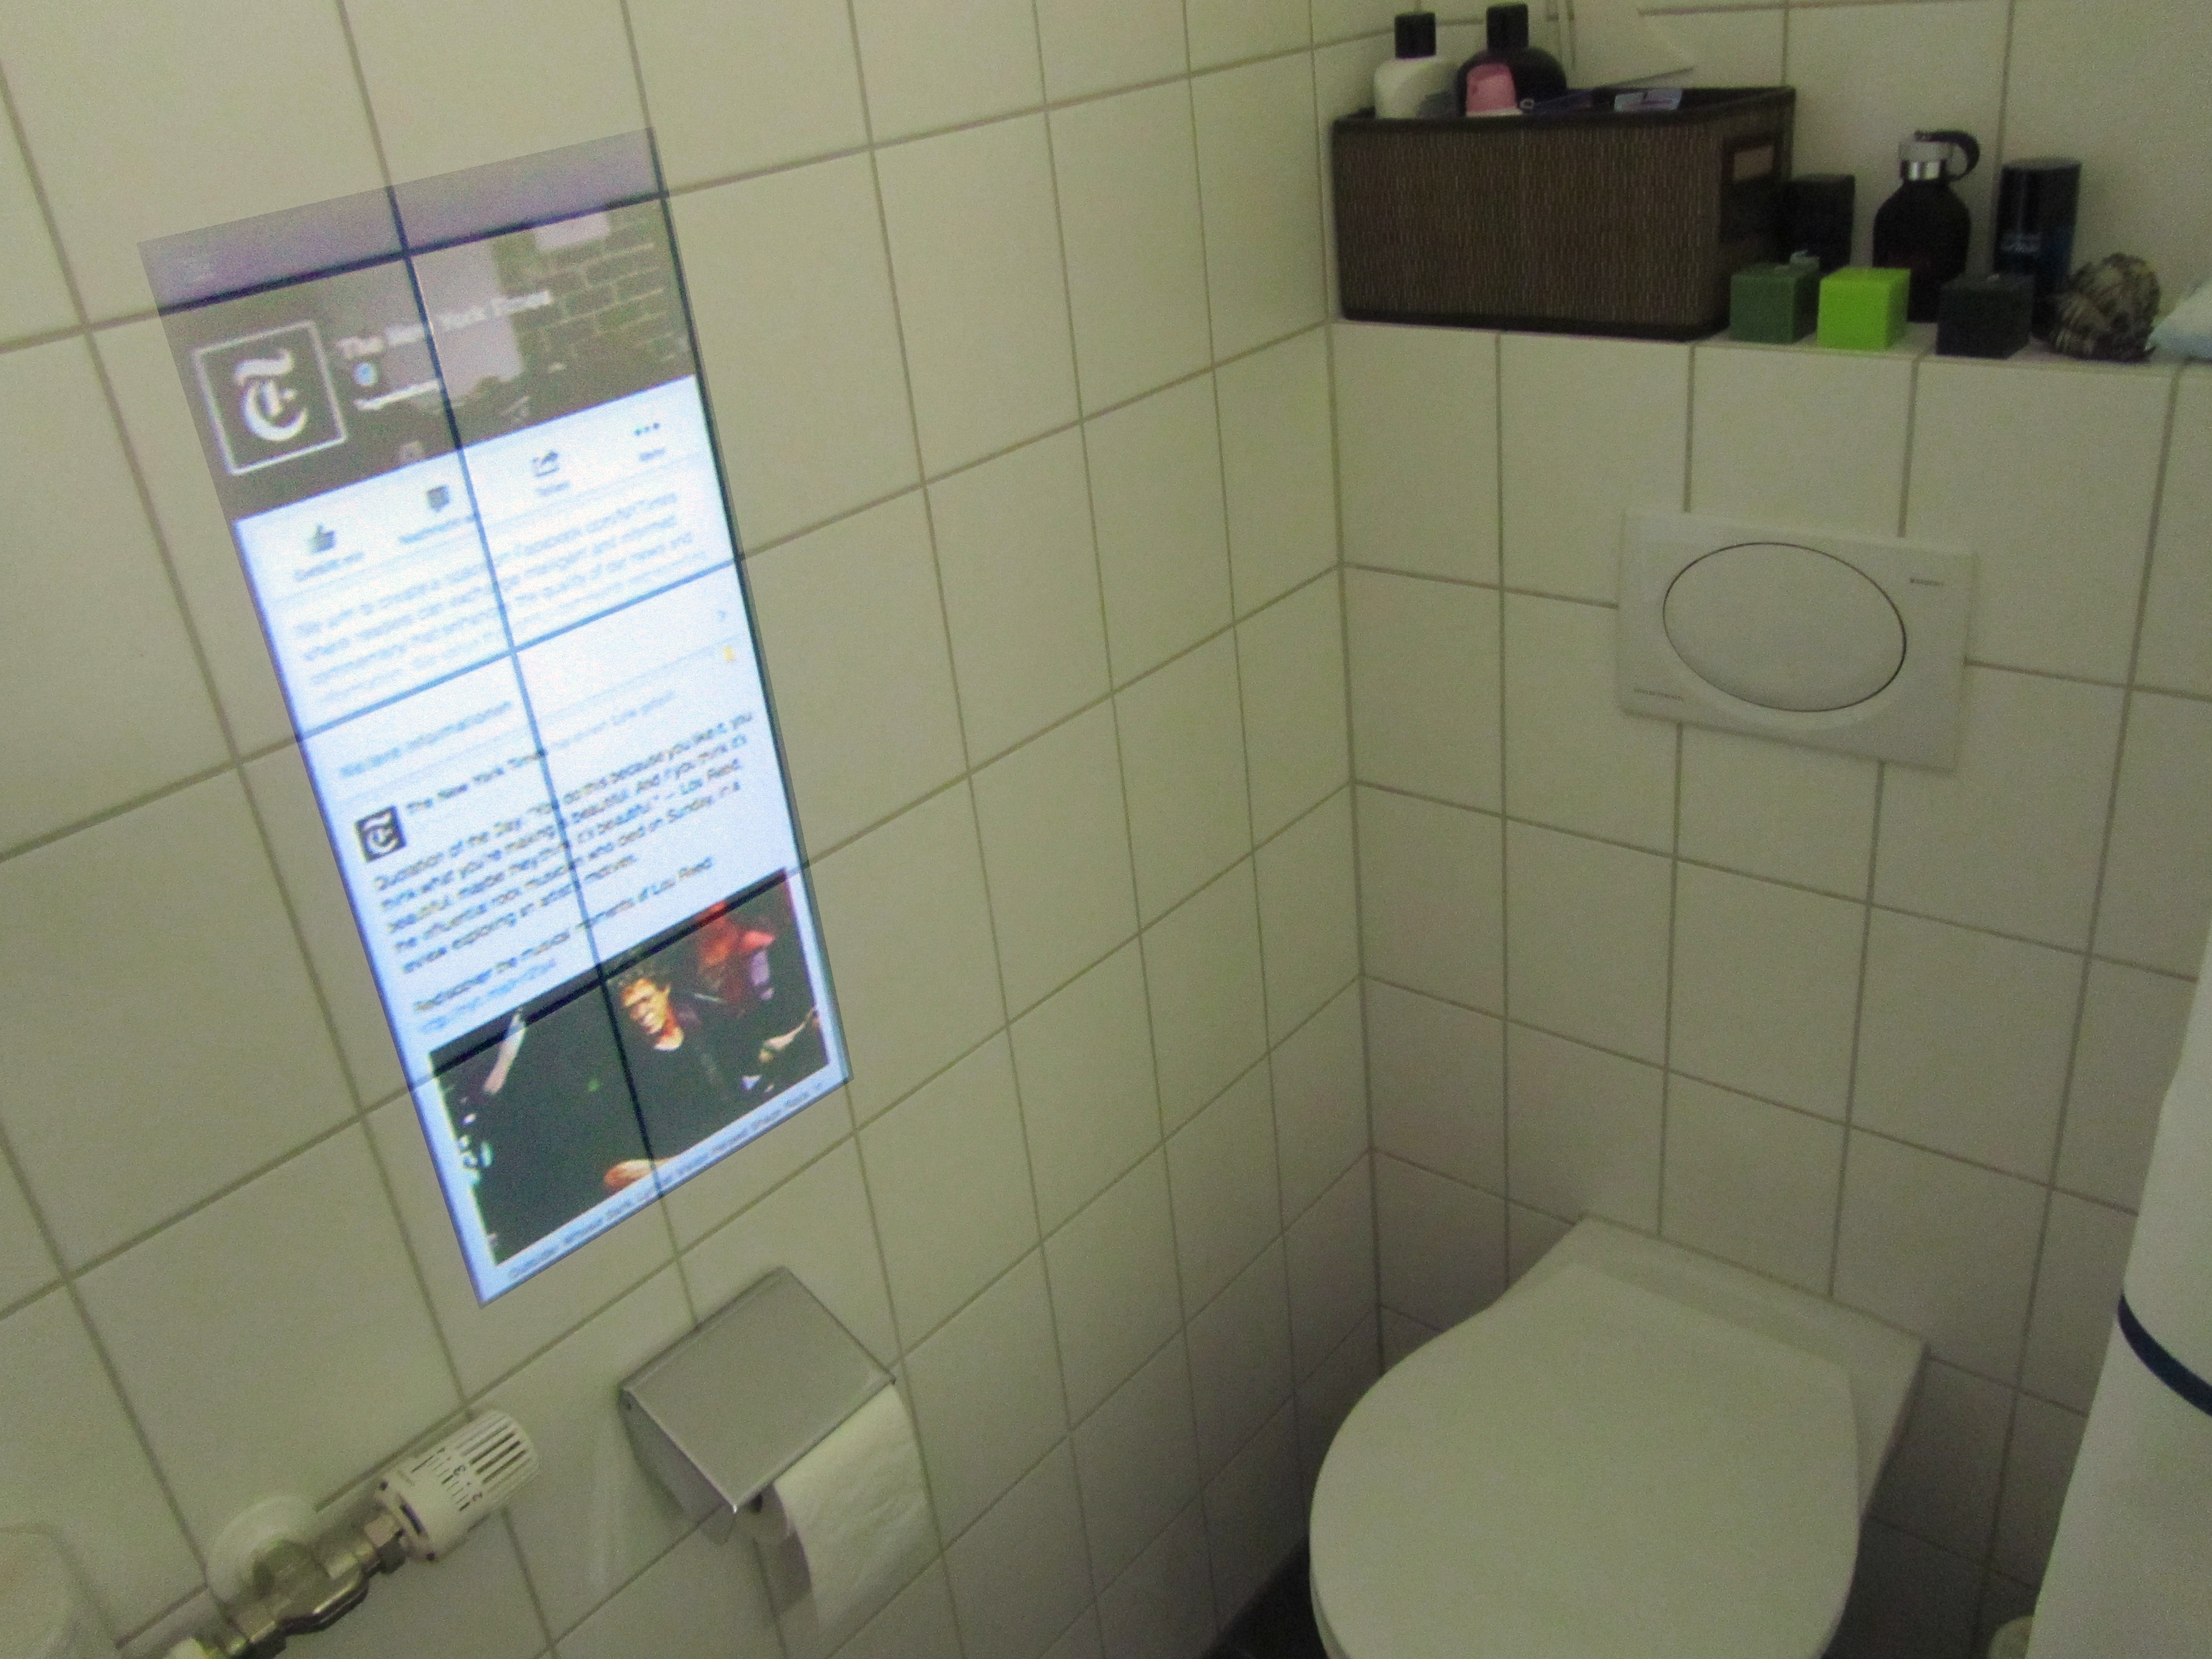
\includegraphics[width=\textwidth]{images/interview/bath02.jpg}
                \caption{Restroom setup}
                \label{img:bath01}
        \end{subfigure}
       \caption{Bath and restroom setup}\label{img:bath}
\end{figure}
In the corridor of the flats participants created \emph{interaction spaces} on free parts of the walls or the doors. One participant also created an \emph{interaction space} on the floor before his front-door to use his doormat as a \emph{surface}. 

\subsection{Placement}
While trying different setups participants always try to mount or place the PROCAMS above body height.
The \ac{PROCAMS} were typically mounted at the ceiling in the centre of the room. Apart from that it was placed on top of higher furniture as cupboards or shelfs. Participants achieved with this kind of placement to minimise the occlusions caused by their bodies when move around the room. 
Dependent on the room size and use case the distance between the \ac{PROCAMS} and the \emph{displays} were \SI{0.7}{\metre} to \SI{3.5}{\metre}. For example only \SI{0.7}{\metre} at the working desk and up to \SI{3.5}{\metre} in the living room when aligned to the large \emph{surface} on the opposite wall of the sofa.

\subsection{Widgets}
Over the course of the interviews, participants propose several widgets. In the kitchen, they describe a widget presenting a digital recipe book. A typical setup using cooking instructions in the kitchen is illustrated in~\autoref{img:cooking2}. 

Another widget which was mentioned several times, especially in the kitchen and working room is a widget which takes track of notes.
In the kitchen in particular a shopping list where items could easily be added and get synchronised with the smart phone was desired. 

Many participants motivate widgets which can be categorised into social media. Especially Facebook and Twitter or pre-configured feeds based on interests were mentioned. Besides social media, a widget presenting news or dynamic information was outlined. In particular global news, weather, sporting news, the TV guide, calendar or the bus timetable were listed. A news widget rendered at the dining table is depicted in~\autoref{fig:newsTable}. Such a widget should also appear, in the vicinity of the user after awaken, to inform him about the latest and upcoming events.

When the PROCAMS is not actively used participants had two ideas how to use the system in an alternative way. On the one hand, they suggested a widget which shows a simple clock or even a combination of different clocks for different time zones. The clock widget should also provide a timer and alarm function to support users while cooking or waking up. This use case is illustrated in~\autoref{img:clock}  On the other hand participants had the idea to use the PROCAMS as an ambient light source. The system could move slowly around and illuminate the room in desired fading colours.

\begin{figure}
        \centering
               \begin{subfigure}[b]{0.31\textwidth}
                \includegraphics[width=\textwidth]{images/interview/kitchen2.jpg}
                \caption{Cooking instruction setup}
                \label{img:cooking2}
        \end{subfigure}
\hfill
        \begin{subfigure}[b]{0.31\textwidth}
                \includegraphics[width=\textwidth]{images/interview/eat.jpg}
                \caption{News on dining table}
                \label{fig:newsTable}
        \end{subfigure}
        \hfill
        \begin{subfigure}[b]{0.31\textwidth}
                \includegraphics[width=\textwidth]{images/interview/kitchen1.jpg}
                \caption{Clock setup}
                \label{img:clock}
        \end{subfigure}
        \caption{Proposed setups and widgets}\label{fig:animals}
\end{figure}

Participants wanted to use the large \emph{surfaces} mainly for two reasons. First they want to replace the television or the media centre with a corresponding widget. Second, especially in the corridor, the \emph{surface} is used to render a digital image frame showing for example the latest holiday photos. In addition, some participant described an interactive music player which visualises the music on the large \emph{display} and presents a control widget in the vicinity of the user e.g. the sofa table. 

Focusing on the sofa table a widget for playing board games was described. Participants wished to combine a projected board with real tokens to play games with dynamic boards. 

Other stated ideas were for instance a digital whiteboard, a widget for action items and a reminder in the working room. Or, a remote control widget for all entertainment devices as a replacement for several different remotes they own.
Four participants also imagined using the \ac{PROCAMS} for home automation purposes or even as video door interphone. Another idea which was mentioned regarding the desk was a widget with shortcuts which could trigger events on the PC. For example, launching the mail application or control the music playback. An interesting last idea only named once, refers to the \emph{display} created at the doormat. A widget should appear there which shows, depending on a status, a away or welcome message.

\subsection{Interaction}
As interaction method participants brought up touch interaction in the first place. It appears to be most obvious interaction concept for interaction with widgets. Secondly they named voice interaction. Participants preferred voice interaction in the kitchen since they need their hands while cooking or they do not want to touch the surface because of dirty hands. Other known concepts mentioned were mid air gestures for scrolling or using a laser pointer to trigger buttons when they are not in the vicinity.

Two participants describe more unique interaction concepts. The first wants to use real physical objects to interact with a widget.  For example, they described a widget showing a counter which increases every time a coffee cup is placed on it. The other wanted to interact via the shadow they produces when the finger is in the light beam of the projector. In particular, this would be usable in some of the bedroom setups where the PROCAMS was close to the user.
Unfortunately, there were no extra novel interaction concepts elaborated. A possible reason could be the well known and daily used touch interaction.


\section{Findings}\label{sec:findings}
During setting up arrangements in the different rooms or final discussion, participants expressed several ideas or ask questions which lead to the following special explanatory notes. While elaborating setups in the bathroom, four participants remark privacy concerns due to the built-in camera. They claimed not to use a PROCAMS in this room. In addition, two participants stated in the bedroom to try to minimise the number of technical devices and therefore would not use a PROCAMS there.

To switch between different \emph{interaction spaces}, the \ac{PROCAMS} should be movable and listen to voice commands or switch to the \emph{surface} the user is tapping on. In total 67\% of the participants want a movable \ac{PROCAMS}. Eight of them propose a PROCAMS, which moves automatically. Four of them want to control by direct manipulation. Furthermore, five participants suggested a battery powered version of a \ac{PROCAMS}. The idea behind it was to enable the possibility to take the \ac{PROCAMS} to friends and share content on a large interactive \emph{display}. Additionally, some participants described the possibility to own only one or two \ac{PROCAMS}, many for financial reasons, which can seamlessly switch between rooms and always know the available \emph{surfaces} and related \emph{displays}. One participant described an intelligent wall plug which takes control of storing \emph{surfaces} for the specific position of the plug and also recharges the portable \ac{PROCAMS} submodule.

Another feature which was mentioned is multi user, multi \emph{display} support. A participant explained that they wanted to use a \emph{display} in a \emph{surface}, for example the kitchen table, while another person can interact with another \emph{display} hosted on the same \emph{surface}.
All participants agreed that the projected widgets need to be in in focus without any interaction. Furthermore, projections have to be light intensive to ensure visibility during daytime.  

For instantiating new \emph{displays} participants explained to use touch gestures or a smart phone as a remote. Further calibration and configuration tasks should not be forwarded to the user, participants said. 

Most participants (10) were satisfied with the dimensions and plain design of the mock-up. Most of the time the PROCAMS will be mounted at the ceiling and is thus not directly in the field of vision. However, some of the participants indicated that they prefer a lighter (3), more robust (1) or more aesthetic (2) version.

\section{Summary}
Interviews with 18 participants were conducted, thereby gaining some new and interesting use cases for a \ac{PROCAMS}. In particular, the wide variety of already existing things which \ac{PROCAMS} can replace is remarkable. Wall paintings, television, clocks, printed bus timetables, alarm clock or a remote control to cite just a few.

Noticeable is that all participants chose only flat \emph{surfaces} even after clarifying that it would be feasible to project without distortion to irregular surfaces. Participants created solutions to get the most of the \ac{PROCAMS} by proposing a movable and straightforward  mount and unmountable system.

On the negative side participants claim about privacy issues.  Some of them also mentioned that depending on the situation parts of the body could occlude larger parts of the display. The overall positive interviews with various ideas lead to some sufficient requirements. Aspiration of the resulting \ac{PROCAMS} is to be available to everyone in a domestic environment.
% !TEX root = ../arbeit.tex
\chapter{Requirements}\label{chapter:requirements}
The build \ac{PROCAMS} is intended to be used by end users in order to investigate their behaviour with everywhere projections. The requirements for this \ac{PROCAMS} are deduced from the findings of the previously accomplished interviews. They are structured in a hardware and software section.

\section{Hardware}
First of all the \ac{PROCAMS} consists of two main components: a projector and a camera. The projector should be lightweight, light intensive and most important have an autofocus, which continuously focuses on the desired \emph{surface}. The camera is necessitate to interact with the \ac{PROCAMS}. To realise simple touch interaction a depth camera is reasonable \cite{Wilson:2010bv,Klompmaker:2012id}.
To achieve a \ac{PROCAMS} which can project to different \emph{interaction spaces} of the room, parts of the system need to be movable. At least the projector and the camera must be able to rotate in two \acl{DOF}. According to 50\% of the participants, alignment  should be possible without any manual effort.


Besides the projector and the camera, the system needs a computational unit which handles at least pre-processing of the camera images, video output to the projector and control of the movement of the unit. Furthermore, there needs to be a wireless link for data transmission as well as a loudspeaker and microphone for audio in- and output. These are the minimum hardware requirements to fulfil the majority of use-cases mentioned in the interviews. A first schematic sketch (see~\autoref{img:sketch}) illustrates how such a system could look like.

\begin{figure}[htbp] 
   \centering
   \includegraphics[width=\textwidth]{images/requirements/sketch_3.pdf} 
   \caption{Schematic sketch of a \ac{PROCAMS}}
   \label{img:sketch}
\end{figure}

\section{Software Framework}
The scope of operation of the hardware is very similar to many other systems \cite{Hardy:2012jo,Xiao:2013dp,Wilson:2012fb,Raskar:2005jy}. But for the user, an efficient working software is as important as a capable and light hardware. To enable frustration-free usability, the system must be usable with a minimum of configuration task. As far as possible configuration and calibration have to be done in the background hidden from the users perspective. For example, after creating a new \emph{interaction space} by aligning the system to the desired space the user should not have to calibrate the system or manually set the focus. All he has to do is to place the \emph{display} to the desired location.

The PROCAMS should be tilted and paned via remote to enable simple changes of the \emph{interaction space}. The space the projector is illuminating. Furthermore, it should be possible to store and load the current settings, including the actual alignment of the system, the position of \emph{displays} and therein rendered widgets. This means that the user is able to load previously stored settings and the \ac{PROCAMS} automatically aligns to this \emph{interaction space} and projects the last shown widgets to the stored positions. In addition, it should be possible to dynamically add and remove \emph{displays} to the \emph{surfaces} without the need to do manual adjustments for a rectified projection.

Development of widgets should be unproblematic and be deployed effortless into the framework in order to enable new rich content. Interaction with widgets should mainly be done via touch input. An alternative input method could be plain speech commands to trigger events like moving to a previously defined \emph{interaction space}. All in all the software framework should disburden the user from unnecessary tasks and allow intuitive use of user-friendly widgets.
% !TEX root = ../arbeit.tex

\chapter{Systems Architecture}
An intuitive to use \ac{PROCAMS} features a tight integration of software and hardware components.
Furthermore, a  fine calibration and well assembled hardware are essential for proficient operation. In the following the architecture design of both, hardware and software, are described in detail.

\section{Hardware Architecture}
The proposed hardware architecture is designed for a compact stand-alone \ac{PROCAMS}. The basis of the systems consists of a camera and a projector. To enable accurate touch detection a depth sensing camera will be used. A motion capture system is no alternative hence it requires an instrumentation of the environment. Such instrumentation would not meet the acquired requirements.
For an easy transformation between the camera and projector coordinate systems, the camera is fixed to the projector. It is important, that the \ac{FOV} of the camera matches the \ac{FOV} of the projector as closely as possible. The projector itself needs to be focus free, as known from laser projectors, or requires the possibility to set the focus electronically via control commands.

Two \ac{DOF} are required to have enough variance to project to any spot visible from the mounting point of the PROCAMS. Thus two rotary actuators are utilised for panning (yaw) and tilting (pitch) of the projector camera unit. The actuator which tilts the unit is bolted directly to the projector. The other is shifted by \SI{90}{\degree} in a vertical plane and bolted to the first actuator. Hereby the projector camera unit is always level. A third actuator which would pivots the unit side to side (roll) is not necessary since it would not change the \emph{interaction space} in a meaningful way.

For a stand-alone solution, the \ac{PROCAMS} includes a powerful processing unit performing all calculations without any remote dependencies. To minimise cable tangle, the processing unit is placed close to the projector and camera. Hence the processing unit is also moving along with the camera and projector. The proposed hardware architecture with a single processing unit for each PROCAMS maximises scalability since no remote connections or calculations are necessary.

An alternative approach using only one powerful dedicated workstation for several PROCAMS is not considered any further. Indeed, the systems could be smaller and lighter since they do not require a processing unit, but this approach will not scale well.
Broadcasting a depth sensing camera video feed for touch detection or elements of the graphical user interface would quickly overstrain the wireless link to the remote unit.

\section{Software Architecture}
Developing a \ac{PROCAMS} fitting the requirements of an average end user is challenging. Technically complex tasks have to be hidden from the user. The initialisation effort has to be minimal while maintaining flexibility. A generic software architecture design for a rotatable \ac{PROCAMS} providing touch input is illustrated in~\autoref{fig:architecture} and described in the following. 

\begin{figure}[htbp] 
   \centering
   \includegraphics[width=\textwidth]{images/architecture/architecture_noshaddow.pdf} 
   \caption{Generic \acl{PROCAMS} software architecture}
   \label{fig:architecture}
\end{figure}

\paragraph{Processing Unit}
The processing unit is the core piece which includes all logic of the \ac{PROCAMS}.
To provide the desired functionality, it requires three input sources. Touch input to control the \ac{GUI}, motion input to control the pan-tilt unit and finally geometry and spatial input for rectified projection to a defined positions in space.

The main task of the processing unit is to collect all these data and performs the necessary calculations to react like the user intends. For example, touch data are reported to the processing unit in a physical world coordinate system. To trigger events on the corresponding widget, touch events have to be transformed to the \ac{GUI} coordinate system regarding the geometry and spatial input. Moreover, the processing unit takes account of all \emph{displays} and rendered widgets. 
To provide dynamic loading of new content or widgets the  processing unit is wirelessly connected to the Internet.
Furthermore, the wireless link is used for receiving remote motion input which is translated by the processing unit and then forwarded to the actuators to control the pan-tilt unit.

\paragraph{User Interface}
For the end user, the \acl{GUI} is the most important part of the \ac{PROCAMS}. In this architecture design, the \ac{GUI} consists of the actual \emph{surfaces} within the \emph{interaction space} the projector is projecting to. Therefore, it is dynamic in terms of spatial alignment. Within a defined \emph{interaction space} widgets can be placed, moved or removed freely on any \emph{surface}. Since the projector is rotatable, \emph{surfaces} are not always planar to the projector. Hence, widgets are encapsulated in \emph{displays} which pre-warps the content to get a rectified reproduction of the widget rendered onto the surface. Geometrically input is used by the processing unit, to calculate the needed transformation to obtain a rectified projection.

\subparagraph{Touch Input} 
Touch input is provided by new smart phones to interact directly by touching the screen with one or more fingers. 
Nowadays, it is a common and well understood input method for users. To enable touch input on ordinary non instrumented surfaces many \ac{PROCAMS}~\cite{Hardy:2012jo,Wilson:2012fb,Xiao:2013dp} use a depth sensing camera to detect touch. Regardless of how the touch is detected, the world coordinates of the detected touch event are passed to the main processing unit. There they are further processed to trigger the desired interaction.  

\paragraph{Motion Input}
Motion input is used to control the alignment of the \ac{PROCAMS}. In order to define a new \emph{interaction space} motion input needs to be provided externally via remote or touch input. Motion input data is passed to the processing unit which triggers the desired events into control commands. Alternatively, stored configuration can be loaded from the database. Control commands are then directly forward the to the actuators. 

\paragraph{Geometry and Spatial Input}
Geometric and spatial input is necessary to gain geometrically and spatially awareness. Geometrically awareness enables the \ac{PROCAMS} to project rectified \ac{GUI} elements to planar or even nonplanar surfaces. Spatial awareness ensures that stored \ac{GUI} elements are always projected to the same position in space. Geometrical and spatial input can be accomplished via tracking or sensing of the environment, or even a combination of both. 

\paragraph{Actuator Control}
Actuator control commands directly power the actuator which rotates the \ac{PROCAMS} or control the focus of the projector when not focus free. Commands are divided into three individual command segments, which are calculated independently by the processing unit. The tilt command segment controls the rotation of the system in the vertical plane. The range needs to be between \SI{0}{\degree} for horizontal alignment to \SI{90}{\degree} for projection onto the floor. As long as the \ac{PROCAMS} is mounted at the ceiling this range is enough to project to the lower hemisphere. The pan command segment is for rotation in the horizontal plane of the \ac{PROCAMS}. A range of at least \SI{360}{\degree} is necessary to cover the complete hemisphere. 
The processing unit translates the motion input or stored \emph{interaction spaces} alignments into actuator control commands to enable projections to all parts of the space.
If a projector is used which requires manual focusing there is an additional control command segment to keep the projection in focus. The processing unit is required to analyse the spatial and geometrical data input and calculate the correspondent focus actuator command.

\paragraph{Storage}
The storage is directly accessed by the processing unit to store and load content, settings and other properties. In particular widgets and  positions. As already described, widgets are relatively simple and easy to use software components which are loaded into the \ac{GUI}. They can vary from simple clock representation, to interactive information presentation or mini games. The other important information which is stored permanently are \emph{positions}. Positions represent the alignment of the \ac{PROCAMS} for a special use case and are separated in a pan and a tilt component. A position property additionally contains the prior projected widgets and their position within the corresponding \emph{display}.
% !TEX root = ../arbeit.tex
\chapter{Hardware Implementation}

Several \acf{PROCAMS} hardware designs have been proposed but often they are bulky, very expensive or need additional environmental instrumentation.
To fulfil the gathered requirements from~\autoref{chapter:requirements} several technologies are evaluated. Focus of attention is on size and quality on the one hand but also the price on the other.
To equip homes with multiple PROCAMSs they need to be affordable.

\section{Actuator}\label{actuator}
Actuators are necessary in order to realise the movement of the \ac{PROCAMS} as well as the automatic focus. There are basically two kinds of electric motors which suit the requirements: stepper motors and servos. 

A stepper motor is a synchronous brushless electric motor.
Rotations are divided into 200 to 400 equal steps. To control the motor, a micro-controller and a additional motor driver is needed. The motor can move step by step or hold the current position. There is no feedback about the current position since the stepper motor has no sensors. For a closed-loop control of the pan-tilt unit, separate sensors are needed, for example an accelerometer and a compass.
Otherwise, the system has to execute a self-calibration each launch to determine the movement constraints and the mapping between steps and position. 

In contrast to a stepper motor, a servo is a combination of an electro motor and a sensor, which provides position and speed feedback.
The position is controlled by a \ac{PWM} signal which can be generated by a micro-controller. The output shaft is moved depending on the difference between the commanded position and the measured position. The position is typically determined by a potentiometer. This allow up to 36000 steps per rotation. Servos are generally used in small robotics. Besides servos for rotational movement, there are also linear moving servos. 

Servo motors with high quality potentiometer offer up to 36000 possible positions per rotation compared to 400 of a stepper motor. Power is only consumed as the servo rotates. A stepper motor continues to consume power while holding a commanded position. As consequence, it runs warm. Finally, stepper motors need additional hardware to control precise positioning. Considering these arguments, using servos as actuators seems to be the superior approach. 

\section{Microcontroller}
A separate microcontroller is needed to command the actuators. When using a servo the microcontroller outputs a \ac{PWM} to set the position of the servo. Using a stepper motor, the microcontroller commands the number of steps to the motor driver.  

A wide variety of microcontrollers which can be used as a servo or stepper motor controller are available. However, embedded programming and an external programmer are necessary. 
The USB IO Board from Hardkernel\footnote{\url{http://www.hardkernel.com/main/products/prdt_info.php?g_code=G135390529643} visited: 02.04.14} allows easy upgrading of the firmware via USB. It provides a PWM interface via a \ac{PIC} microcontroller. Nevertheless, low level programming is required. 

Boards like the IOIO-OTG\footnote{\url{http://ytai-mer.blogspot.de/2013/01/go-go-ioio-on-go.html} visited: 02.04.14}, mainly developed by Ytai Ben-Tsvi, provide similar interfaces. The IOIO-OTG is especially designed to work with Android devices. A Java based API offers abstract and lucid programming. With such a board and the provided API neither low level programming nor an external programmer is necessary. 

Another platform offering effortless microcontroller programming is Arduino \cite{Arduino:b6u8ceDY}. It is an open-source prototyping platform combining software and hardware. Many boards in different sizes and versions are available to suit different use-cases. Whereas, hardware design is open-source there are also less expensive boards from third-party manufacturers obtainable. The microcontroller is programmed with a platform independent IDE based on the Processing IDE. Various Arduino libraries are linked to simplify C and C++ programming. The servo library for example, allows setting the position of the servo with one simple command. Regarding these arguments, Arduino is used as microcontroller platform. 

\section{Projector}
Projection technologies became more sophisticated over the years. New technologies allow smaller and less power consuming devices. Projectors can be classified by light source and projection technology. Typically light sources are laser, LED, arc lamps and combinations of laser and LED. Arc lamps consume much power and become very hot. So, they require a powerful cooling system which makes them loud and bulky. Therefor, projectors with an arc lamp are not further examined.

There are three major projection technologies utilising lasers as light source \cite{Mertens:p40QFV-L}. With Laser-Beam-Steering the image is created pixel by pixel by a laser beam guided across the projection surface by using a mirror. Combining three lasers with different colours (red, green, blue) and intensity using optics, a full coloured image is created. Light Blue Optics \cite{Blue:2014ab} developed Holographic Laser Projection where a laser illuminates a hologram that diffracts the laser to create the original image. Light Blue Optics claim, that it is very power efficient and has less speckle than other laser projector technologies. A new technology combines lasers and \ac{LCoS} to project an image. White laser light as a combination of red, blue and green is used to illuminate the \ac{LCoS}, which control the amount of reflected light by changing polarisation. Research showed \cite{Guttag:2011wd} that with this approach more eye safety, lower power consumption and higher resolution are possible. All three technologies using laser light have the advantage that the image is always in focus. No manual refocusing is necessary. However, maximum brightness of laser projectors is 50 ANSI Lumen which requires a dimmed environment for acceptable visibility. 

One of the most mature technologies using LEDs as light source is \ac{DLP} developed by Texas Instruments \cite{Rukzio:2012hj}.
Light is emitted to tiny mirrors on a chip that directs the light. Dependent on the state, light is reflected to the surface or an absorber. Colour is generated by a rotating colour wheel splitting the light into red, blue and green. The above described technology using \ac{LCoS} is also used with LEDs, but this time focusing optics are necessary. Since LEDs are not getting very hot while operating, small and energy efficient projectors with LEDs are available. While maximal brightness of tiny laser projectors is limited to 50 Lumen, LEDs projectors provide up to 550 lumen without exceeding the size of half cubic decimetre.

\section{Depth Sensing Camera}\label{sec:depthsensingcamera}
Three distinct technologies are applicable to generate depth information~\cite{Ko:2012vp}. Stereoscopic vision systems use two slightly offset cameras and compare the obtained images. On basis of the difference in location of a point in corresponding images, the depth can be calculated. Stereoscopic vision systems are very low-cost but high in software complexity. The depth accuracy is only in the cm range. 

Depth sensing cameras using \ac{SL} pattern have also high software complexity but offer, dependent on the model, depth accuracy in \textmu m to cm range. In comparisons to a stereoscopic vision system, one camera is replaced by a laser or led light source which creates a light pattern. This pattern is obtained by the remaining camera. To acquire depth information the same technique is used, but due to the pattern, finding corresponding points is easier and more accurate.

A relatively new technology is \ac{ToF}. It allows depth accuracy in the mm range. An emitter transmits a light pulse to an object. There it gets reflected and finally determined again by the receiver. The distance of an object can be calculated by measuring the time between transmit and receive of the light pulse. Available \ac{ToF} cameras have only a quarter of pixel resolution compared to \ac{SL} cameras. But temporal resolution with up to 160 \ac{fps} (Argos 3D - P100) is very high.

\begin{table}[htb]
\begin{tabularx}{\textwidth}{ l X l l p{1.9cm} p{1.9cm}}
\toprule
Type & Tech-nology & Range (m) & FOV (H,V) & Depth res. (w x h,fps) & Colour res. (w x h,fps) \\
\midrule
Kinect XBOX & SL & 0.8 - 10.0 & 57.0, 43.0 & 640x480,30 & 1280x960,12 \\
Kinect Windows & SL & 0.4 - 3.0 & 57.0, 43.0 & 640x480,30 & 1280x960,12 \\
Kinect 2 & ToF & 0.8 - 4.0 & 70.0, 60.0 & 512x424,30 & 1920x1080,30 \\
Carmine 1.08 & SL & 0.8 - 3.5 & 57.5, 45.0 & 640x480,60 & 640x480,60 \\
Carmine 1.09 & SL & 0.35 - 1.4 & 57.5, 45.0 & 640x480,60 & 640x480,60 \\
DS311 short & ToF & 0.15 - 1.0 & 57.3, 42.0 & 160x120,60 & 640x480 \\
DS311 long & ToF & 1.5 - 4.5 & 57.3, 42.0 & 160x120,60 & 640x480 \\
DS325 & ToF & 0.15 - 1.0 & 74.0, 58.0 & 320x240,60 & 1280x720 \\
Senz3D & ToF & 0.15 - 1.0 & 74.0, 58.0 & 320x240,30 & 1280x720 \\
\bottomrule
\end{tabularx}
\caption{Depth sensing camera overview.}
\label{tab:cams}
\end{table}
In~\autoref{tab:cams} a brief overview of several commercially available depth sensing cameras is given. 
In late 2013, Apple bought PrimeSense the manufacturer of the Carmine cameras. Ever since PrimeSense cameras are no longer available for purchase.
The DepthSense311 (DS311) and DS325 are developed by SoftKinetic a Belgian company. The Kinect and Kinect 2 is manufactured by Microsoft, but by now it is not possible to develop applications with the Kinect 2. Senz3D bases on the DepthSense311 and is made available by Creative.
	


\subsection*{SDKs and Frameworks}\label{sec:depthSDK}
Hardware manufacturers distribute powerful SDKs to minimise the challenges in developing frameworks or applications which their depth sensing cameras. Moreover, there is a big community developing frameworks, offering numerous useful functionalities and services.

The Kinect SDK is used to develop Kinect-enabled applications. It includes Kinect Fusion and  Kinect Interactions. With Kinect Fusion it is possible to create a 3D reconstruction of objects or the environment in real time. Kinect Interaction provides gesture recognition. iisu, an acronym for ''The Interface Is You``, is the 3D gesture recognition development framework by SoftKinetic. As well as Kinect SDK it supports full body tracking and natural gesture development and recognition. Intel Perceptual Computing SDK supports body and gesture recognition as well as facial analysis, hand and finger tracking. The SDK focuses on short range interaction in particular. \ac{OpenNI} is an open source SDK for middleware and application development mainly driven by PrimeSense. The framework supports voice and voice command recognition, hand gestures and full body motion tracking. The point cloud library (PCL) is an open source library which offers many algorithms for n-dimensional point could processing. In the context of depth sensing, the provided algorithms like filtering, surface reconstruction, or segmentation allow sophisticated analysis of the scenery.~\autoref{tab:depthFrameworks} summarises which depth sensing camera receives the support of which framework.
\begin{table}[htb]
\vspace{4em}
\centering
\begin{tabular}{r|ccccc} &
\begin{rotate}{60} OpenNI \end{rotate} &
\begin{rotate}{60} Kinect SDK  \end{rotate} &
\begin{rotate}{60} Intel PC SDK  \end{rotate} &
\begin{rotate}{60} IISU  \end{rotate} &
\begin{rotate}{60} PCL \end{rotate} \\ \hline
Kinect        & \CIRCLE  &   \CIRCLE 	 &  \Circle    	& \CIRCLE    & \CIRCLE  \\
Kinect 2        & \Circle      &   \LEFTcircle  &  \Circle    	& \Circle       & \Circle  \\
Carmine        & \CIRCLE  &   \Circle   	 &  \CIRCLE  	& \CIRCLE   &  \CIRCLE\\ 
DepthSense  & \Circle     &   \Circle   	 &  \CIRCLE  	&\CIRCLE   &\Circle \\ 
Senz3D	     & \CIRCLE  & \Circle  		&  \CIRCLE	& \CIRCLE  & \CIRCLE	\\
\hline
\end{tabular}
\caption{Overview of supported SDKs. \\\CIRCLE supported  \Circle not supported  \LEFTcircle announced}
\label{tab:depthFrameworks}
\end{table}



\section{Single Board Computer}\label{sec:sbc}
The hardware design of the proposed stand-alone PROCAMS includes a processing unit which is fixed near to the projector and camera. The processing unit needs to be small and lightweight. To connect WiFi, microcontroller and the depth sensing camera, at least three USB-ports are mandatory. These requirements lead to a so called \ac{SBC}, a complete computer built on a single circuit board. To handle all computations a high performance SBC is essential. An overview of currently existing SBC is given in~\autoref{tab:sbc}.
It should be noted that most of the high performance SBC utilise the ARM \ac{ISA}. Deduced from mobile phone processors, SBC processors are very energy efficient, produce little heat and have similar computational power as present mobile phones. 
However, using the ARM architecture narrows the choice of \acfp{OS} to Linux and Android.

\begin{table}[htb]
\begin{tabularx}{\textwidth}{ l l X l X l l}
\toprule
NAME & CPU (GHz) & RAM (MB) & USB & SIZE (cm) & \acs{ISA} & \acs{OS} \\
\midrule
 ODROID-XU & 4x(1.6 + 1.2) & 2048 & 4/2 & 7x9.4 & ARM & L, A \\
 ODROID-X2  & 4x1.7 & 2048 & 6 & 9x9.4 & ARM & L, A \\
 ODROID-U2 & 4x1.7 & 2048 & 2 & 4.8x5.2 & ARM & L, A \\
 Origen Board & 4x1.4 & 1024 & 2 & 11.9x11.9 & ARM & L, A \\
 Arndale Board & 2x1.7 & 1024 & 3 & 36x24 & ARM & L, A \\
 Nitrogen6X & 4x1 & 1024 & 2 & 11.4x7.6 & ARM & L, A, W-CE \\
 Sabre Lite  & 4x1 & 1024 & 2 & 8.25x8.25 & ARM & L, A, W-CE \\
 Via Epia-P910 & 4x1 & 512 & 2 & 10x7.2 & X86 & W, X, L, A \\
\bottomrule
\end{tabularx}

\caption{Single-board computer overview. Operating system acronyms: \textbf{L}inux, \textbf{A}ndroid, OS \textbf{X}, \textbf{W}indows and  \textbf{W}indows-\textbf{CE}}
\label{tab:sbc}
\end{table}

\section{Used Hardware}
\paragraph{Actuator}
For pan and tilt of the PROCAMS two HS-785HB by HiTEC are used. This are quarter scale servos with a torque of \SI{132}{\N\cm} at \SI{6}{\volt}. They are one of the stronger servos in this size segment. Based on the data sheet, a full rotation takes less than \SI{9}{\second}.
Focus is driven by a NYA 2.9g linear long throw servo SPMSH2040L from Spektrum with a torque of 329g running at \SI{4.2}{\volt}.

\paragraph{Microcontroller}
Actuators are controlled by an Arduino Pro Mini. This is one of the smallest Arduino boards. It is built on the ATmega168 with six PWM output pins for servo control. Arduino is used because it offers great library support for servo control as well es easy prototyping. 

\paragraph{Projector}
For the proposed PROCAMS the ultra-compact LED projector ML550 by OPTOMA is used. In this projector, DLP technology by Texas Instruments combined with a LED light source is deployed. It measures only \SI{105 x 106 x 39}{\mm} in size and weights \SI{380}{\g}. The projection distance is between \SI{0.55}{\meter} and \SI{3.23}{\meter}.

\paragraph{Depth Sensing Camera}
The depth sensing cameras presented in~\autoref{sec:depthsensingcamera} can be divided into short (less than 1.4 metres) and long distance sensing cameras. Derived from the interviews, a long distance sensing camera is necessary. For deployment, the Carmine 1.08 from PrimeSense was chosen. It has a smaller form factor than the Kinect and a higher depth resolution than the DS311. Moreover, it is supported by all presented Frameworks except the Kinect SDK.  

\paragraph{Single Board Computer}
As processing unit, the ODROID-XU was chosen. It is developed by Hardkernel a South Korean open source hardware company. ODROID-XU is one of the most powerful SBC available. The CPU is based on big.LITTLE architecture which features a powerful eight-core for efficient handling of multitasking. Besides it has enough ports to connect the Android Pro Mini microcontroller, the depth sensing camera as well as a WiFi-Dongle and keyboard. 


\section{Pan-Tilt Unit}
The pan-tilt unit is responsible for moving the complete PROCAMS, in detail the depth sensing camera, the projector and the SBC. 
There are commercially available pan-tilt units e.g. the D46-17build by FLIR or the MPT1100-SS retailed by ServoCity. However, these products are heavy, large in size and expensive. Prises are around 650 to 2500 USD. Tending to an affordable lightweight stand-alone \ac{PROCAMS}, an approach with servo motors looks promising. A direct drive mechanism without any reductions minimises additional gearing and bearing parts.

\pagebreak
Each of the tilt and pan servo is grounded to a \textit{ServoBlocks} by ServoCity. A ServoBlocks isolates the lateral load from the servo and increase the load-bearing. ServoBlocks are easily screwed together to create rigid structures actuated by servos.  An image of a servo fixed to a \textit{ServoBlocks} is illustrated in~\autoref{img:servo}.

\TwoFig{images/hardware/servo.jpg}      {ServoBlocks construction}                  {img:servo}
       {images/hardware/pantilt.png}{Pan-Tilt unit}{img:pantilt} {Hardwar and construction of pan-tilt unit} {}
       
The pan servo is mounted overhead. To gain more open space for tilting, a 3D-printed \ac{PLA} spacer (see~\autoref{img:spacer}) is connected to the hub shaft. The tilt servos is rotated by \SI{90}{\degree} in a vertical plane. The hub shaft is bolted to the other side of the spacer. A complete illustration of the pan-tilt unit is shown in~\autoref{img:pantilt}.
\begin{table}[htb]
\begin{tabularx}{\textwidth}{ X p{2cm} X l}
\toprule
Command  & Code & Value & Description \\
\midrule
Position & 00 & - & Returns pan and tilt value \\
Pan & 01 & Position in \textmu s & Pan to given position \\
Tilt & 02 & Position in \textmu s & Tilt to given position \\
Focus & 03 & Position in \textmu s & Focus to given position \\
\midrule
Up & 04 & - & Moves unit up \\
Down & 06 & - & Moves unit down \\
Left & 05 & - & Moves unit left \\
Right & 07 & - & Moves unit right \\
\bottomrule
\end{tabularx}
\caption{Implemented commands for pan-tilt unit and focus control}
\label{tab:arduinoCommands}
\end{table}
\pagebreak
The servos are controlled by the previous presented Arduino Mini Pro. The Arduino framework provides a servo library which allows simple servo control. Via serial interface the ODROID-UX SBC can send commands to the Arduino board which are translated into servo control commands.  Commands are seperated into command code, and optional values. Code and values are separated by a \# character. The command to pan to a specific direction for example is:  \verb+pan#position+ respectively \verb+01#1580+ where position is the pulse width in \textmu s. All supported commands are summarised in~\autoref{tab:arduinoCommands}. 

\begin{figure}[htbp]
        \centering
        \begin{subfigure}[b]{0.3\textwidth}
                \includegraphics[width=\textwidth]{images/cad/spacer.png}
                \caption{Pan-Tilt unit spacer}
                \label{img:spacer}
        \end{subfigure}
        \quad
        \begin{subfigure}[b]{0.3\textwidth}
                \includegraphics[width=\textwidth]{images/cad/focus.png}
                \caption{Focus handle grabber}
                \label{img:focusHandle}
        \end{subfigure}
         \quad
         \begin{subfigure}[b]{0.3\textwidth}
                \includegraphics[width=\textwidth]{images/cad/servo.png}
                \caption{Focus servo mount}
                \label{fig:focusServo}
        \end{subfigure}
        \caption{3D-representations of the special designed parts}
\end{figure}

\section{Focus}
% !TEX root = ../arbeit.tex
\begin{wrapfigure}{r}{0.5\textwidth}
\vspace{-1em}
  \centering
\begin{tikzpicture}
	\begin{axis}[
    /pgf/number format/.cd,
        1000 sep={},
        		height=.5\textwidth,
		width=.5\textwidth,
		grid=major,
		legend pos=south east,
		xlabel=Distance,
		ylabel=PWM sig. in \textmu s,
	]	
	\addplot[draw=blue][domain=55:285] {-36076/x + 1750};
	\addlegendentry{model}
	\addplot coordinates {
(60,1130)
(72,1230)
(80,1330)
(100,	1430)
(140,1480)
(190,1530)
(280,1630)};
	\addlegendentry{measurement}
	\end{axis}
	\end{tikzpicture}
         \caption{Focus-Distance model}

\label{plot:focus}
\end{wrapfigure}
The focus of the Optoma 550ML is manually adjusted via a small lever. To realise automatic adjustment of the focus, the movement of the lever must be controlled with a servo. A linear servo is used for this task. The servo is glued to the designed servo mount shown in~\autoref{fig:focusServo}. This construction is then glued to the projector, left of the adjustment lever. A special piece is designed (see~\autoref{img:focusHandle}) which grabs the lever and is also connected via a steel wire to the servo. The complete construction is illustrated in~\autoref{fig:autofocus}. The servo is controlled in the same way as pan and tilt servo.

To determine the required position of the servo for a given distance a calibration task was conducted. The projector was placed at seven different distances between \SI{0.6} and \SI{2.8}{\meter} perpendicular to a wall. The corresponding PWM signal that produces the visually sharpest focus was determined. These seven distance--PWM value pairs were used to determine the formula for setting the focus. Non-linear regression with two parameters was used for analysis.
Analysis leads to:
\begin{equation}
\nonumber
\notag
\mathit{PWM}=\frac{-36076.6267}{distance} + 1750.06825
\end{equation}
Where $\mathit{PWM}$ is the PWM signal in \textmu s and  $distance$  is the distance between surface and projector in cm. The measured values and the calculated formula are plotted in~\autoref{plot:focus}. Maximum error is less than 40\textmu s which does not lead to projections which are out of focus.

\begin{figure}[htbp]
        \centering
        \begin{subfigure}[b]{0.61\textwidth}
                \includegraphics[width=\textwidth]{images/hardware/focus.png}
          	\caption{Autofocus construction}
         	\label{fig:autofocus}
        \end{subfigure}
          \hfill
        \begin{subfigure}[b]{0.31\textwidth}
                \includegraphics[width=\textwidth]{images/cad/case.png}
                \caption{Projector and SBC case}
                \label{img:projectorCase}
        \end{subfigure}
        \caption{Hardware construction}\label{img:cad}
\end{figure}
	
\section{Construction}
After assembling the pan-tilt unit and preparing the auto focus, the complete hardware of the PROCAMS is assembled and wired. To connect the projector and SBC with the pan-tilt unit a special case (see~\autoref{img:projectorCase}) is designed and 3D-printed. The PrimeSense depth sensing camera is glued to the bottom of the projector facing the same direction with a maximum overlap of both fields of views. The final hardware construction is illustrated in~\autoref{img:finalConstruction}. 

It measures only \SI{10.5 x 12.2 x 22.5}{\cm} including the pan-tilt unit and weights \SI{996}{\g}. With a size of \SI{10.5x12.2x9}{\cm} excluding the protrude part of the camera and a weight of about \SI{690}{\g} the PROCAS itself (excluding the pan-tilt unit) is notable smaller and lighter.
The complete hardware can be bought and assembled for less than 1000 USD, assuming mechanical skill and access to a 3D printer. 

\begin{sidewaysfigure}[h] 
\centering 
                \includegraphics[width=\textwidth]{images/hardware/constructionFull.png}
                \caption{Complete construction of the stand-alone PROCAMS}
                \label{img:finalConstruction}
\end{sidewaysfigure}
% !TEX root = ../arbeit.tex
\chapter{Software Implementation}
Building a stand-alone \acf{PROCAMS} requires a lightweight and resource saving software. Processing power provided by the ODROID-UX presented in \autoref{sec:sbc} can not stick with current workstations. For a responsive user interface experience, developed algorithms have to be adjusted to the available hardware resources.

As mentioned earlier the ODROID-UX builds on ARM architecture. Linux and Android are natively supported. There continues to be no Windows support for the ARM architecture for researchers. Following a guide\footnote{\url{http://forum.odroid.com/viewtopic.php?f=61\&t=2207\&p=16999\#p16999}}, Ubuntu 12.04 was installed to this relatively new hardware. Some special changes to the video driver and kernel were necessary. Ubuntu was chosen since it is lightweight and has a great library support for different tasks.  
For reading RGB and depth images, OpenNI version 2.2 for ARM \cite{Anonymous:5lF7gVK2} introduced in \autoref{sec:depthSDK} is used. Image processing is done with OpenCV in version 2.4.6 \cite{Intel:H9HpU8rd}. OpenCV is an open source library aiming at real time computer vision algorithms. Visualisation of widgets is accomplished with Qt (version 4.8.2) \cite{Digia:BVAEvJrQ}, a library for UI development using C++ and QML. 

The developed software can be separated into five packages.
\begin{description}
\item[Touch Detection] Detecting direct user input.
\item[Transformation] Mapping of touch events to UI elements.
\item[Pan-Tilt Unit] Receiving user input and controlling pan-tilt unit.
\item[User Interface] Rendering of rectified widgets to surfaces.
\item[Main Logic] Loop handling all events and PROCAMS logic.
\end{description}

\section{Interaction}
Interaction with the PROCAMS is divided into three intuitive parts. First, initial alignment of the projector to create the \emph{interaction space}. In other words where the projection should appear. Secondly placing and arranging the UI-elements namely widgets. And finally, the interaction with widgets itself. The first two tasks are basically one time actions since different alignments of the PROCAMS and the arrangement of widgets are stored. This allows undemanding switching between several surfaces for different use-cases.

The PROCAMS is designed to be ceiling-mounted. Hence, direct manipulation of the alignment is not possible. 
A remote control to control the alignment of the PROCAMS is implemented based on suggested ideas from the interviews. The user is able to control the pan-tilt unit and in this way the alignment of the projection via their smart phone. An Android-App displaying a virtual joystick allows indirect  manipulation as well as storing and loading previous configurations. 

After the configuration of the location, the system executes a self-calibration task. This task is concealed from the user and takes only a short period of time. Then, the PROCAMS can be operated via touch interaction. Following interactions are provided: 
 
\begin{description}
\item[Adding Widgets]  \hfill \\
The user can add widgets by touching and holding the surface at a free spot. A menu with the available widgets appears and the user can choose one of them. The widget is then projected rectified at the previously touched position. Of course, it is possible to add more than one widget to the \emph{interaction space}. 

\item[Moving Widgets] \hfill \\
The user can rearrange the widget by touching and holding (long press) the widget until a red frame appears. When moving the finger around the widget sticks it. When done, the user just presses the green check button and the red frame disappears.

\item[Removing Widgets]\hfill \\
To remove a widget the user long presses on it. When the red frame appears a trash icon on the right side of it needs to be pressed to remove the widget.
\end{description}

After arranging all widgets to the desired layout the user can interact with them immediately. Widgets can offer any content to the user. The current implemented framework forwards four different touch events to the widget. Implemented events are touch down, touch move, long touch and touch release. However, more sophisticated interaction like multi-touch, size and number of touches or the like \cite{Xiao:2013dp} can be easily added to the framework.


\section{Touch Detection}
Accurate and responsive touch detection is a crucial part of this thesis. There are several frameworks \cite{FORTHFoundationforResearchTechnologyHellas:F3nqLAGA,Klompmaker:2012id} and projects \cite{Hardy:2012jo,Xiao:2013dp} supporting finger tracking or touch detection, but all require high performance workstations. Additionally, CUDA (Compute Unified Device Architecture), a parallel computing platform by NVIDIA giving direct access to the GPU processing, or the .NET Framework by Microsoft is required to gain reasonable results. \textcite{FORTHFoundationforResearchTechnologyHellas:F3nqLAGA} developed tracking runs only at 2.67 \ac{fps} on an Intel Core 2 Duo with 2.20GHz and 4096 MBs of RAM using a Quadro FX 1600M for example. Neither CUDA nor .Net is supported by the used SBC. 

For that reasons a unique very lightweight touch detection, based on the research of \textcite{Wilson:2010bv} is developed. A key feature is that touch is detected on any physical object without user driven calibration tasks. 
The developed touch detection can be separated into four parts. First the scenery is analysed and a spatial image, the ground truth, is generated. This obtained image is used to calculate a binary contact image while touch detection is running. The contact image is filtered and simple blob detection detects contact points. In a last step, contact points are tracked over time and transformed into interaction events which finally trigger events intended by the user. 

\begin{figure}[htbp]
        \centering
        \begin{subfigure}[b]{0.31\textwidth}
                \includegraphics[width=\textwidth]{images/software/gt/RGBImage.jpg}
                \caption{RGB image of scenery}
                \label{img:rgbGT}
        \end{subfigure}
        \hfill
        \begin{subfigure}[b]{0.31\textwidth}
                \includegraphics[width=\textwidth]{images/software/gt/actualImage.jpg}
                \caption{Single depth image}
                \label{img:depthGTSingle}
        \end{subfigure}
         \hfill
         \begin{subfigure}[b]{0.31\textwidth}
                \includegraphics[width=\textwidth]{images/software/gt/GroundTruth.jpg}
                \caption{Filtered ground truth}
                \label{img:GTtemp}
        \end{subfigure}
        \caption{Calculating ground truth}
        \label{img:calcGT}
\end{figure}

The spatial ground truth image is generated by temporal filtering of 30 single depth images. First a dilation operation with a structuring element of 7x7 in size is executed on the depth image. For each pixel depth information is cumulated and divided by the number of depth information available. As result, a good noise reduced approximation of the scenery is calculated. Temporal and spatial filtering is necessary since the depth sensing camera provides only noticeable noisy depth information. A single depth image is shown in~\autoref{img:depthGTSingle} and the corresponding filtered ground truth in~\autoref{img:GTtemp}. Depth information are encoded from near (light grey) to far (dark grey). Black pixel provide no depth information because depth is out of sensing range or because of noise.

A simple assumption is made to enable fast contact image calculation. If the current depth for a pixel is less than the corresponding pixel in the ground truth (minus some offset) and is beyond greater than the ground truth minus the height of a finger, the pixel is representing a potential contact point. This coherence is illustrated in~\autoref{img:finger}. 
\begin{figure}[htbp]
\begin{center}
                \includegraphics[width=.6\textwidth]{images/software/finger.png}
\caption{Concept of contact point calculation \cite{Wilson:2010bv}}
\label{img:finger}
\end{center}
\end{figure}

Where $d_{surface}$ is the depth in the ground truth image, $d_{max}$ is $d_{surface}-\mathit{offset}$. The $\mathit{offset}$ needs to be well chosen to minimise false positives due to noise. $d_{min}$ is $d_{surface}-\mathit{finger}$. The $\mathit{finger}$ value specifies in which height from the surface a contact is detected. Mathematical a pixel $d(x,y)$ is a potential contact point if the following formula holds:
\begin{equation*}
d_{max}(x,y) > d(x,y) > d_{min}(x,y)
\end{equation*}

A contact point image is illustrated in~\autoref{img:cpT}. Since there are still some false positives the image needs to be filtered before a blob detection can be executed. Therefore a low-pass 3x3 box filter and subsequent thresholding is applied. 
For performance reasons the box filter is separated into one 1x3 respectively 3x1 filter. Separating the filter leads to faster filtering by more than 40\%. A filtered contact point image is shown in~\autoref{img:fcpT}
On this filtered image a blob detection is executed. First the \textit{SimpleBlobDetector} of the OpenCV framework was applied, but it proved to be too slow. Analysing one frame takes between 45 and 58 ms which is far from realtime. Hence, an alternative library namely OpenCVBlobsLib\footnote{\url{http://opencvblobslib.github.io/opencvblobslib/}} is utilised. This library makes use of multi core processing and analyses an image in less than 6ms. The result of a blob detection is illustrated in ~\autoref{img:rgbT} and~\autoref{img:blobdetectT}. Detected blobs are marked green in these images.

\begin{figure}[htb]
        \centering
        \begin{subfigure}[b]{0.48\textwidth}
                \includegraphics[width=\textwidth]{images/software/no_touch/RGBImage165644_comob.jpg}
                \caption{Image with detected touch points}
                \label{img:rgbT}
        \end{subfigure}
    \hfill
        \begin{subfigure}[b]{0.48\textwidth}
                \includegraphics[width=\textwidth]{images/software/no_touch/actualImage.jpg}
                \caption{Depth image for touch detection}
                \label{img:depthT}
        \end{subfigure}        
               
      \vspace{1em}

        \begin{subfigure}[b]{0.31\textwidth}
                \includegraphics[width=\textwidth]{images/software/no_touch/initalDiffImage.jpg}
                \caption{Potential contact points}
                \label{img:cpT}
        \end{subfigure}
     \hfill
        \begin{subfigure}[b]{0.31\textwidth}
                \includegraphics[width=\textwidth]{images/software/no_touch/filteredDiffImage.jpg}
                \caption{Filtered contact points}
                \label{img:fcpT}
        \end{subfigure}
        \hfill
         \begin{subfigure}[b]{0.31\textwidth}
                \includegraphics[width=\textwidth]{images/software/no_touch/blobs.jpg}
                \caption{Detected blobs}
                \label{img:blobdetectT}
        \end{subfigure}
        \caption{Touch detection sequence showing two touching fingers and one hovering hand.}
        \label{img:calcGT}
\end{figure}
Due to the prior analysis of the scenery, contact points can be detected on any random shaped surface as long as the depth sensing camera can see it. This allows in particular simultaneous touch detection on diverse aligned surfaces. 

Detected contact points are tracked over time to classify them into different touch events. As described prior events are touch down, touch move, touch release and long touch. The implemented tracker assigns the $\mathit{time}$
of the first appearance, $\mathit{age}=0$  and $\mathit{lives} = 5$ to each new detected blob. In subsequent frames distances between previous blobs and the new blobs are calculated. If the distance is below a certain threshold, the $\mathit{age}$ for this particular blob is increased. Additionally, the distance is cumulated and stored in $\mathit{movement}$. This is used for long touch detection.  
For all previous blobs, where no corresponding blob is found, the $\mathit{lives}$ is decreased. All new blobs are handled like described before. Touch events are differentiated as following: 

\[
    \mathit{event}= 
\begin{cases}
    \text{touch down},& \text{if }  \mathit{age} = 3 \\
    \text{long touch}, & \text{if } \mathit{age} > 3 \wedge \mathit{movement}<\mathit{thld}_{move} \wedge \mathit{time}_{elapsed} =  {thld}_{time}\\
    \text{move}, & \text{if } \mathit{age} > 3\\
    \text{touch release},& \text{if } \mathit{age}  \geq 3 \wedge \mathit{lives} =0\\   
    \text{no event},& \text{otherwise}
\end{cases}
\]
Where $\mathit{thld}_{move}$ is the threshold for the maximum allowed distance the finger can drift whereby a long press is still detected and $\mathit{time}_{elapsed}$ is the time a long press takes.

The position of a touch event is detected in the depth sensing camera coordinate system. Whereas all \ac{GUI} elements also known as widgets are located in the projector coordinate system. Hence, event coordinates need to be transformed to the projectors coordinate system. This transformation procedure is outlined in the next section.

\section{Calibration and Transformations}
Mapping the detected touch event coordinates from the camera coordinate system to the widget, displaying the content, is necessary to enable interaction at all. Therefore, the touch event point $P_{x,y}$ detected in the camera coordinate system is transformed several times until the point is located in the same coordinate systems as the widget. In detail, the touch point is transformed from the depth sensing camera coordinate system to the colour camera coordinate system. From there to the world coordinate system which is the only three dimensional coordinate system in the transformation process. From the world coordinate system, the point can be transformed to the projectors coordinate system. There it is transformed one last time to the widgets coordinate system since it is pre-warped. This many transformations are indispensable because only the transformation matrixes between the named coordinate systems are known or can be determined due to manual one time calibration task.

\subsection{Camera-Projector Calibration}
The most challenging part is to determine the transformation between the depth sensing coordinate system and the projectors one. \textcite{Xiao:2013dp} present an approach to determine the perspective transformation between a Kinect and a projector, but a special 3D-calibration target is needed. Hence, such a target was not accessible other approaches were evaluated. 
Simple colour-camera-projector calibration algorithms are developed by \textcite{LegardaSaenz:2004hn,Gao:2008jn,Li:2008kr} using structured light or \textcite{Ashdown:2005dx,Griesser:2006ko,Audet:2009ee} using optical pattern.

Using the colour camera for camera projector calibration requires to transform the touch point from the depth sensing coordinate system to the one of the colour camera. Despite that, an additional concept for calibration presented by~\textcite{Audet:2009ee} was chosen. Especially because he provides a software, ProCamCalib\footnote{\url{http://www.ok.ctrl.titech.ac.jp/~saudet/research/procamcalib/}}, which performs a ``full calibration of a camera and a projector in about 30 second'' by preserving comparable good results as the preceding stated concepts. 

To use the ProCamCalib software a special \textit{framegrabber} was implemented since the software was originally developed for simple web-cameras and not for depth sensing cameras. The OpenNI framework was used to read colour frames from the PrimeSense camera. The frames were then transformed in a ProCamCalib readable format.

\begin{figure}[htbp]
        \centering
        \begin{subfigure}[b]{0.486\textwidth}
                \includegraphics[width=\textwidth]{images/software/barcode.png}
                \caption{Printed barcode pattern}
                \label{img:patternCalib}
        \end{subfigure}
    \hfill
        \begin{subfigure}[b]{0.46\textwidth}
                \includegraphics[width=\textwidth]{images/software/calib.png}
                \caption{Calibration process}
                \label{img:calibCam}
        \end{subfigure}        
        \caption{Projector camera calibration with printed and projected barcode pattern}
        \label{img:calibrationproces}
\end{figure}
Indeed, the calibration task itself is really simple. The printed pattern containing fiducial markers (shown in~\autoref{img:patternCalib}) enables the software to calculate the intrinsic parameters of the camera. Then the projector starts to project an inverted  marker pattern into the spaces of the printed one which the camera tries to recognise (see~\autoref{img:calibCam}) simultaneously. The intrinsic parameters of the projector can be calculated when the projected pattern is detected. Knowing this information the software takes several pictures showing the pattern in different poses and calculates the extrinsic parameters which reflect the relation between the camera and the projector. With this information touch points can be transformed from the camera coordinate system into the 3D world coordinate system and then into the projectors one. The calculated calibration file for the built PROCAMS is printed in~\autoref{apx:calib}.

\subsection{Transformation}
As mentioned, several transformations are necessary to calculate the position of the touch event represented in the widgets coordinate system. In the following, the executed transformations are described in detail. 

\subsubsection{Depth Sensing Camera - Colour Camera}
The transformation between depth sensing camera and colour camera is necessary since the calibration was performed between colour camera and projector. Fortunately, the OpenNI framework in combination with the used PrimeSense camera allows a direct mapping of the depth sensing camera image to the colour camera image. This is done internally by the camera hardware so no computational performance is wasted. 

\subsubsection{Colour Camera - World}
The $3\times4$ camera matrix describes the mapping from 3D points in world space to 2D points in a camera image. It is identified in the calibration task. Using the inverse camera matrix as well as the camera distortion coefficients which contains the intrinsic parameters allow in combination the distance from the depth sensing camera a retransformation of the touch point into the 3D world coordinate system. For matrix multiplication and rectification, OpenCV library is used. 

\subsubsection{World - Projector}
Transforming the point from the  3D world coordinate system into the projector space is the inverse operation to the colour camera - world transformation using the projectors parameter. This time the projector matrix containing the alignment of the projector in the world coordinate system as well as the projectors distortion coefficients are used to calculate to perspective projection of the 3D point onto the projector image. This operation is also performed using the  OpenCV library. 

\subsubsection{Projector - Widget}
Since the widget is pre-warped to enable a rectified projection the touch point needs to be transformed once again.
The transformation of the widget is set out in~\autoref{sec:widget}. Since the perspective transformations matrix which is applied to the widget is known, the touch point can be transformed in the same manner. 

Finally, the coordinate of the touched point is known and the interaction can be performed as designated by the widget. 
	
\section{Pan-Tilt Unit Control}
\begin{wrapfigure}{r}{0.5\textwidth}
		\vspace{-2em}
  		\begin{center}
                	\includegraphics[width=.42\textwidth]{images/software/android_template.png}
  		\end{center}
		  \vspace{-1em}
		  \setcapindent{0pt}
		  \captionsetup{width=0.42\textwidth}
\caption{Android App providing control over the PROCAMS pan-tilt unit via joystick}
	\label{img:appUi}
       \vspace{-3em}    
\end{wrapfigure}

The user can execute the initial alignment of the PROCAMS remotely. An Android App was implemented to provide basic control of the pan-tilt unit. The App UI is shown in~\autoref{img:appUi}. It consists of a virtual joystick and four buttons for storing and loading surface configurations as well as starting interaction and recalibrating. Moving the joystick on the display triggers the pan-tilt unit to move the PROCAMS to the desired direction. Meanwhile, the projector is rendering a frame indicating the resulting \textit{interaction space}

The App connects via Internet to the server running on the PROCAMS. The server receives the movement commands (up, down, left, right) and forwards them via serial interface to the connected Arduino microcontroller which handles the movement of the servos. The check button triggers the self-calibration task for the touch detection and starts the system for user interaction. The recalibrate button provides the opportunity to repeat the calibration task if for example the touch detection ground truth run out of sync due to unintentional movement of the PROCAMS. Pressing the store button asks the user to provide a name for the current configuration. The store command and the name are then transmitted to the server which stores name, current position of the PROCAMS as well as the position of the widgets in a database. On pressing the load button all stored positions are loaded from the server and displayed to the user for selection.

\section{User-Interface} 
After setting up the alignment of the PROCAMS and self-calibration of the touch detection is done the user can start placing widgets. The interaction space is still indicated by a light white frame.

The projector is usually not aligned perpendicular to the surface it is projecting to. This causes geometrical distortion. 
Rendering a representation of the widgets without distortion onto the surfaces requires a pre-warping according to the alignment of the projector to the surface.


\subsection{User-Interface Pre-Warping}
For the proposed PROCAMS, the already available depth map, the ground truth calculated for touch detection, is used to facilitate a rectified projection. First a plane detection is executed on the depth map to find possible projection surfaces. Then four points situated on one of the detected planes, spanning a rectangle of the desired size are determined. Finally, the affine transformation which transforms the widget to the determined points is calculated and applied to render a corrected representation of the widget. These three steps will now be described in detail.

\paragraph{Plane Detection} 
Plane detection is done following the concepts \textcite{Yoo:2013he} presented in their work. To compute the surface normal of a point $P_{x,y}$ in the ground truth depth map, four points with a distance $d$ around the point are selected. Up: $P_{x,y-d}$, Down: $P_{x,y+d}$, Left: $P_{x-d,y}$ and Right: $P_{x+d,y}$. $d$ defines the amount of smoothing. A greater $d$ will flatten the surface normal since it is calculated over a larger area. These four points are transformed into world space and the vectors between up-down and left-right are determined (see~\autoref{img:normalsCalculation}). The cross product of these two vectors is finally the surface normal $N_{x,y}$ of the point $P_{x,y}$.

\begin{figure}[htpb]
        \centering
        \begin{subfigure}[b]{0.31\textwidth}
	      \centering
               \def\svgwidth{.78\textwidth}
               \import{images/software/ui/}{dmap2.pdf_tex}
                \caption{Surface normals calculation scheme \cite{Yoo:2013he}}
                \label{img:normalsCalculation}
        \end{subfigure}
         \hfill
                  \begin{subfigure}[b]{0.31\textwidth}      
                \includegraphics[width=\textwidth]{images/software/gt/GroundTruth.jpg}
                \caption{Depth map of scenery\newline}
                \label{img:normalGT}
        \end{subfigure}
         \hfill
         \begin{subfigure}[b]{0.31\textwidth}      
                \includegraphics[width=\textwidth]{images/software/gt/normalsImage_mod_2.jpg}
                \caption{Colour encoded surface normals}
                \label{img:normals}
        \end{subfigure}
        \caption{Plane detection}\label{fig:animals}
\end{figure}
Surface normals are directly calculated after determination of the ground truth in the self-calibration task. To minimise processing time surface normals are only calculated over a grid with a distance of 4x4 pixel. For a given ground truth like illustrated in~\autoref{img:normalGT} the corresponding surface normals are presented in~\autoref{img:normals}. The length of each direction (X,Y,Z) of the normal vector $N_{x,y}$ is encoded via a corresponding colour (red,green,blue). Hence, surface normals pointing in the same direction have the same colour. 


\paragraph{Rectangle Calculation}
When the user presses long at the surface to add a new widget, the position as well as the surface normal in camera-space is known. 
Both define a plane where the widget should appear rectified. Therefore, the plane (point and normal) is transformed into world space. Based on the normal vector, two vectors $x$ and $y$ each perpendicular to each other and to $N_{x,y}$ are calculated. Hence the alignment of the pan-tilt unit is known $x$ and $y$ can be rotated in that way, that $y$ points down and $x$ is horizontal  in the 3D coordinate system. The calculated vectors are displayed in red and blue in~\autoref{img:vectors}. 

\begin{figure}[htpb]
        \centering
               \def\svgwidth{.35\textwidth}
               \import{images/software/rectify/}{surface_2text.pdf_tex}
                \caption{Surface normals calculation in world-space}
                \label{img:vectors}
\end{figure}
Knowing the two vectors, allows to calculate the four vertexes of the rectangle where the widget should appear. 
The four points can be calculated as follows:

\begin{equation*}
\begin{split}
\text{P}_0 & = P_{x,y} \\
 \text{P}_1 & = P_{x,y} +w\times x  \\ 
\text{P}_2 & = P_{x,y} + h\times y \\
 \text{P}_3 & = P_{x,y} + w\times x + h\times y   \\ 
\end{split}
\end{equation*}

Where $P_{x,y}$ is the point the user touched, $w$ the width and $h$ the height of the desired widget. These four points in the 3D world coordinate system are then transformed into the projector coordinate system  in order to calculate the perspective transformation for the widget.

\paragraph{Projective Transformation}

Projective transformation allows creating perspective distortion. This is needed to change the perspective of the projected content in order to get an undistorted representation of the content. The conceptual result of a projective transformation is visualised in~\autoref{img:projectionGrid}.
\begin{figure}[htbp]
\begin{center}
	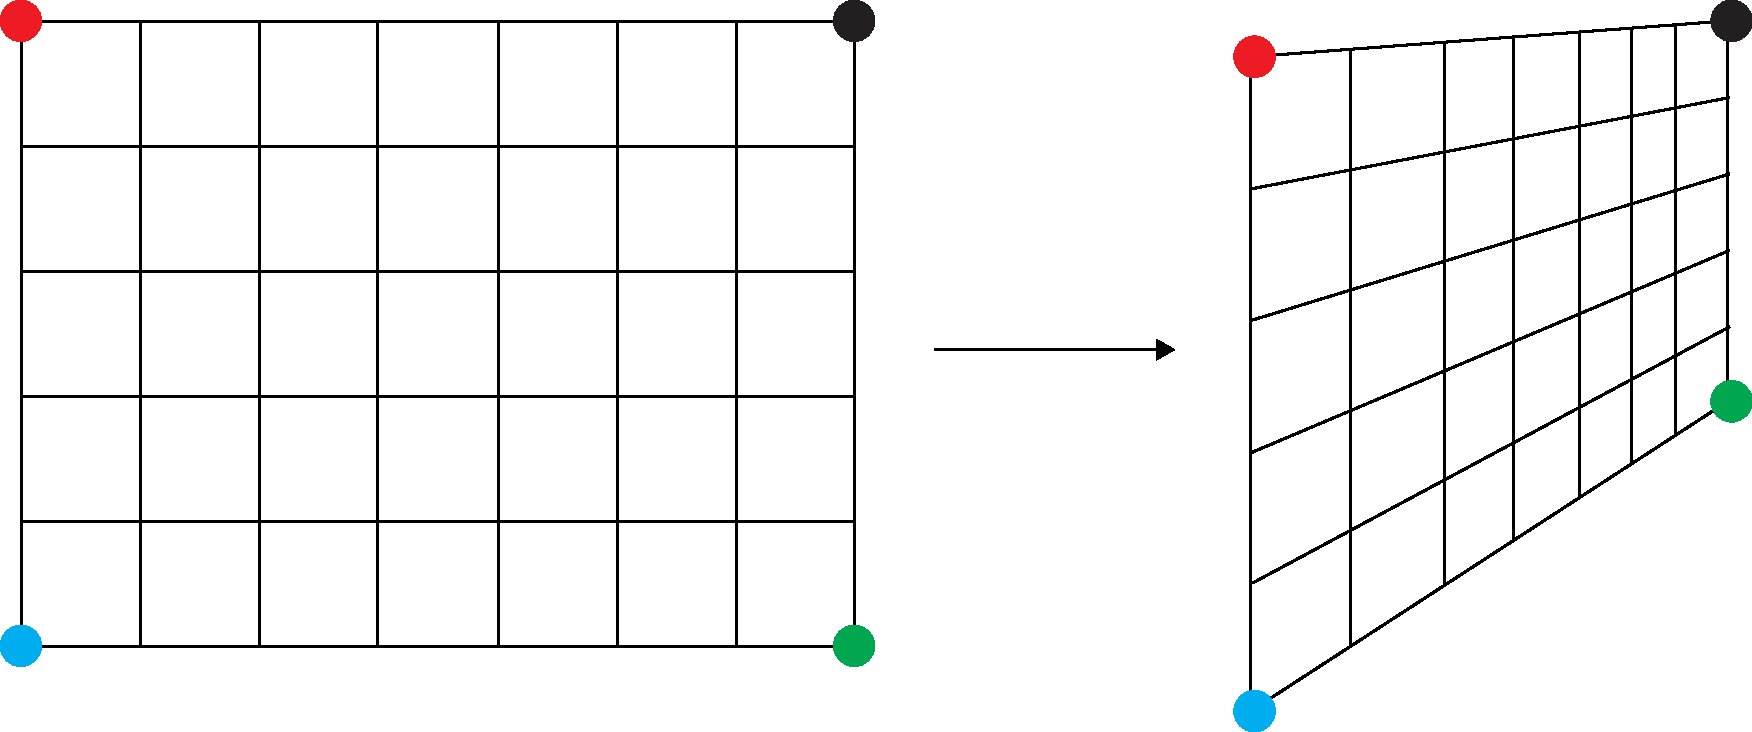
\includegraphics[width=\textwidth]{images/software/transformation/perspectiveTransformation.pdf}
\caption{Projective transformation}
\label{img:projectionGrid}
\end{center}
\end{figure}

Projective transformation are realised by simple matrix multiplication:
\begin{equation*}
\begin{pmatrix}
a_1 & a_2 & b_1  \\
a_3 & a_4 & b_2  \\
c_1 & c_2 & 1
\end{pmatrix}
\times
\begin{pmatrix}
x  \\
y  \\
1
\end{pmatrix}
=
\begin{pmatrix}
x'  \\
y'  \\
1
\end{pmatrix}
\end{equation*}

Where $a_1$ to $a_4$ is the rotational matrix which performs scaling and rotation, $t_1$ and $t_2$ is the translation vector, moving the content in space, and $c_1$ and $c_2$ is the projection vector. $x$ and $y$ are the source positions which are projected to $x'$ and $y'$.  

With the four prior calculated and transformed points it is possible to determine the projective transformation matrix so that the vertex of the content e.g. the widget with defined vertex points at position (0,0), (1,0), (0,1) and (1,1), are transformed to the calculated ones. 
The transformation of an exemplary clock widget as well as the projected rectified result is shown in~\autoref{img:SimpleWarpClock}. For calculating the transformation matrix the \textit{QTransformation} class provided by Qt was utilised. Calculation starting from the ground truth is done fully automatic without any interaction necessary by the user. 
\begin{figure}[htbp]
        \centering
        \begin{subfigure}[b]{0.27\textwidth}
                \includegraphics[width=\textwidth]{images/software/clock_3.png}
                \caption{Simple clock Widget}
                \label{img:SimpleWarpClock1}
        \end{subfigure}%
         \hfill 
         \begin{subfigure}[b]{0.27\textwidth}
                \includegraphics[width=\textwidth]{images/software/clock_warped.png}
                \caption{Pre-warped widget}
                \label{img:SimpleWarpClock2}
        \end{subfigure}
         \hfill
        \begin{subfigure}[b]{0.36\textwidth}
                \includegraphics[width=\textwidth]{images/software/clock_project.jpg}
                \caption{Widget projected on surface}
                \label{img:SimpleWarpClock3}
        \end{subfigure}
        \caption{Pre-warping of a widget}\label{img:SimpleWarpClock}
\end{figure}

\pagebreak
\subsection{Widgets}\label{sec:widget}
The developed framework allows dynamic loading of widgets which actually displays the content to the user. 
All the complexity of the spatially aware projection, dynamic touch detection and movement of the PROCAMS are encapsulated and hidden from the view of the widget. This enables trouble-free and straight forward widget development. 

Two different possibilities are supported to create a new widget. Developers are able to implement the provided interface depicted in~\autoref{widgetCodeListing} to create a more desktop like looking widgets. The interface inherits from \textit{QWidget} the base class of all Qt user interfaces. The interaction logic can directly be implemented in the corresponding methods. In the \textit{paintEvent} method, the projected representation of the widget must be implemented. The core logic of the widget can be implemented as desired, for example by following the model view controller pattern.

Alternatively, developers can implement widgets using \ac{Qt Quick}. It uses QML to describe modern looking, fluid UIs in a declarative manner. Qt Quick is increasingly used on mobile phones or other embedded hardware.
QML allows to develop the logic using Javascript or even native code. Simplicity is shown by the source code (printed in~\autoref{QMLCodeListing}) for a plain widget showing a scrollable web page.
In both cases, widgets can easily be developed and tested in a common desktop environment by simply deploying them as a desktop application. This allows rapid creation of rich widgets without the need of the PROCAMS nearby. In addition, there are a lot of tutorials, demos and sample widgets provided by Qt Project \cite{Digia:BVAEvJrQ} which all run directly or after just small modifications in the framework.
\begin{figure}[htbp]
        \centering
        \begin{subfigure}[b]{0.235\textwidth}
                \includegraphics[width=\textwidth]{images/software/bus.png}
                \caption{Timetable widget}
                \label{img:wid:bus}
        \end{subfigure}
	\hfill
        \begin{subfigure}[b]{0.38\textwidth}
                \fbox{\includegraphics[width=\textwidth]{images/software/gnews.png}}
                \caption{Google News widget}
                \label{img:wid:news}
        \end{subfigure}
	\hfill
        \begin{subfigure}[b]{0.28\textwidth}
                \includegraphics[width=\textwidth]{images/software/clock.png}
                \caption{Qt clock widget}
                \label{img:wid:time}
        \end{subfigure}
        \caption{Some implemented widgets}
        \label{fig:Widgets}
\end{figure}

Three widgets were implemented. A simple digital image frame which shows dynamically loaded images. On touching the left or right part of the image, the next or previous image is presented. The second widget is an adaptive bus time table (see~\autoref{img:wid:bus}) which shows the next buses leaving a desired bus stop. The last implemented widget is a news browser (see~\autoref{img:wid:news}), showing the Google news website. Any other web page could be displayed by this widget as well.
In addition, three widgets provided as demos by Qt Project were slightly modified to work with the proposed framework. The first one is a simple clock showing the time (see~\autoref{img:wid:time}), the second one is a sophisticated image browser allowing to browse the flickr.com image library in a convincing way. The third adapted widget shows a Twitter feed. There are many more examples available offering great services. Most of them can directly deployed into the developed framework. The three exemplary chosen widgets conduce just as proof of concept.
% !TEX root = ../arbeit.tex
\chapter{Evaluation}\label{chapter:evaluation}
To validate the fineness and quality of the proposed PROCAMS a technical evaluation was executed. In particular, the precision and speed of the pan-tilt unit were examined as well as the touch accuracy. Finally, overall performance of the PROCAMS is evaluated.
While planning the execution of larger usability studies in a domestic environment this evaluation should give a first clue of strengths and weaknesses of the build PROCAMS. 

\section{Pan-Tilt Unit Performance}
The task of the pan-tilt unit is to move the PROCAMS fast and accurate to a desired location. This two properties accuracy and pace were assessed in a laboratory study.

\subsection{Alignment Accuracy}
The accuracy approaching a previously stored position was determined by placing the PROCAMS with a distance of \SI{1}{\m} to a wall. The projector was displaying a red cross to indicate the centre of the projection. Then the pan-tilt unit was commanded to approach the stored position from eight defined starting points. The position where the red cross came to a standstill was marked at the wall.
Starting points were up, up-right, right, right-down, down, down-left, left, and left-up. Where up and down indicates a vertical shift by \SI{45}{\degree} from the stored position. Accordingly left and right indicates a horizontal shift by \SI{90}{\degree}. The measured distances in horizontal a vertical direction between the marked and stored position lead to an angel of aberration by simple trigonometry.
The stored position was approached ten times from each starting point. Thus 80 data points were obtained. A plot of the data is shown in~\autoref{plot:movement}.
% !TEX root = ../arbeit.tex
\begin{figure}[htbp]
        \centering
\tikzset{mark options={mark size=2, line width=1.5pt}}
\begin{tikzpicture}
	\begin{axis}[%
	width=\textwidth,
	height = .6\textwidth,
	xmax = 6.5,
	xmin = -5.5,
	xstep= 1,
	ymin = -2.5,
	ymax =3.5,
	ystep=1,
	grid=major,
	legend columns=4,
	xlabel=Horizontal aberration in degree,
	ylabel=Vertical aberration in degree,
	scatter/classes={
		Up={mark=x,yellow},
		Up-Right={mark=x,blue},
		Right={mark=x,gray},
		Right-Down={mark=x,magenta},
		Down={mark=x,green},
		Down-Left={mark=x,orange},
		Left={mark=x,red},
		Left-Up={mark=x,black}
		}]
	\addplot[scatter,only marks,%
		scatter src=explicit symbolic]%
	table[meta=label] {
x     y      label
-4.67424872612533	1.40704466542326			Up
-3.93360909963853	1.40704466542326			Up
-3.1916505442666	1.40704466542326			Up
-2.9631282497019	0.834310816061917			Up
-2.50580769586769	1.40704466542326			Up
-1.87648177481699	2.09394419785448			Up
-2.50580769586769	2.66590922345048			Up
-3.59131574999252	3.12310419675389			Up
-3.1916505442666	3.12310419675389			Up
-2.50580769586769	2.66590922345048			Up
4.87197278490512	3.12310419675389			Up-Right
4.70128244616578	1.922268042484			Up-Right
5.04257648050957	1.8650348309974			Up-Right
5.32671540617036	1.8650348309974			Up-Right
5.44029823293142	1.23524883003786			Up-Right
5.66733440279074	1.23524883003786			Up-Right
5.83749482341844	1.29251672941418			Up-Right
4.70128244616578	1.29251672941418			Up-Right
4.92885045666407	1.29251672941418			Up-Right
3.56135251033059	1.29251672941418			Up-Right
5.83749482341844	-0.8844333423724			Right
5.49707362345356	-0.5407128664187			Right
5.55383818745301	-0.483421668036623			Right
6.23412919364215	-0.598002983536637			Right
5.950877911401	-0.254248352762198			Right
6.00755197509656	-0.311542730726946			Right
5.950877911401	0.0322288725769704			Right
5.950877911401	0.0895245826339467			Right
5.83749482341844	0.375998155486819			Right
5.04257648050957	0.146820113642666			Right
2.13256625938215	-2.08679175426757			Right-Down
3.33299828852148	-2.02956988177023			Right-Down
2.18978055419555	-1.74340203526284			Right-Down
1.27390493988743	-1.39988698938846			Right-Down
1.27390493988743	-1.45714715525241			Right-Down
1.67470826450442	-1.17081949820428			Right-Down
2.30419592354254	-1.17081949820428			Right-Down
2.18978055419555	-0.655291904866927			Right-Down
4.47356567736875	-1.9151140985677			Right-Down
2.53297060324095	-2.02956988177023			Right-Down
-4.90183476990765	-1.9151140985677			Down
-4.56039979299942	-1.9151140985677			Down
-4.33259451138178	-1.9723439586187			Down
-4.27562145717918	-2.14400946240445			Down
-3.64838313294688	-1.80064302302008			Down
-3.53424123132033	-1.62890972945458			Down
-3.1916505442666	-0.483421668036623			Down
-1.18943272767241	-1.22809016670015			Down
-0.444749555610536	-0.655291904866927			Down
-4.0476456276837	-1.68615756608216			Down
-2.44861895803739	-2.20122289252437			Down-Left
-2.04816744014753	-2.25843193102194			Down-Left
-1.76200574367305	-2.08679175426757			Down-Left
-2.7345115584368	-1.34262402653776			Down-Left
-2.62017007131273	-1.34262402653776			Down-Left
-2.50580769586769	-1.39988698938846			Down-Left
-2.33422694871262	-1.45714715525241			Down-Left
-2.04816744014753	-1.39988698938846			Down-Left
-1.76200574367305	-1.39988698938846			Down-Left
-1.93371422794441	-1.28535838089828			Down-Left
-2.62017007131273	-0.712579515900411			Left
-2.50580769586769	-0.941714567461968			Left
-2.33422694871262	-0.8844333423724			Left
-1.93371422794441	-0.8844333423724			Left
-1.76200574367305	-0.8844333423724			Left
-2.39142533786276	-1.34262402653776			Left
-1.93371422794441	-1.22809016670015			Left
-2.39142533786276	-0.426129502926883			Left
-2.04816744014753	-0.426129502926883			Left
-2.33422694871262	-0.998993909972118			Left
-2.62017007131273	0.261410180165005			Left-Up
-1.70476239345517	0.891593594551635			Left-Up
-2.67734348248654	1.5215613564293			Left-Up
-1.70476239345517	1.6360658892936			Left-Up
-1.99094282098346	2.09394419785448			Left-Up
-2.1053879716975	2.15116137745379			Left-Up
-2.33422694871262	3.1802267828006			Left-Up
-2.44861895803739	3.29445285887791			Left-Up
-2.50580769586769	3.40865272433571			Left-Up
-1.93371422794441	3.40865272433571			Left-Up
	};

\addlegendentry{Up}
\addlegendentry{Up-Right}
\addlegendentry{Right}
\addlegendentry{Right-Down}
\addlegendentry{Down}
\addlegendentry{Down-Left}
\addlegendentry{Left}
\addlegendentry{Left-Up}

	\end{axis}
\end{tikzpicture}
\caption{Aberration of the pan-tilt unit approaching a defined location}
\label{plot:movement}
\end{figure}

The average horizontal misalignment is \SI{3,29}{\degree}. For vertical alignment, the average error is \SI{1,48}{\degree}. Hence, the misalignment in an arbitrary direction is \SI{3,74}{\degree}. This accords to a shift of less than \SI{10}{\cm} if the \emph{surface} is \SI{150}{\cm} away from the projector.
A likely reason for the smaller misalignment in the vertical direction is caused by an additionally used accelerometer to control the servo for horizontal alignment. Since, for horizontal alignment no secondary sensor is used, the alignment is not as good. Overall the alignment is fair enough to re-project a widget at almost the same location in the physical world, but is not sufficient enough to augment small tangible objects as for example a light switch. 

A more accurate alignment could be achieved by two different modifications. On the one hand, a sensor providing very accurate data for horizontal and vertical alignment could be attached to provide feedback of the current alignment of the pan-tilt unit. Nonetheless, previous attempts already showed that a simple calibrated and compensated compass is not suitable for this task since the projector and servos have a strong influence on the magnetic field.

On the other hand, more powerful servos with a high resolution potentiometer could be installed. The potentiometer would lead the servo to move more precisely to the commanded position. This approach seems very promising without any major change at the pan-tilt unit. 

\subsection{Alignment Pace}
The pace of the pan-tilt unit was evaluated in a separate benchmark. Therefor, the time needed for \SI{164}{\degree} horizontal pan and a \SI{110}{\degree} tilt was measured. Each movement was repeated ten times from both directions. Since panning and tilting is performed simultaneously no combinations of tilt and pan were executed.

On average the pan-tilt unit needed \SI{3.5}{\second} for the horizontal pan task. For the tilt task, the unit needed \SI{4.8}{\second}. A reason for the slower tilt movement could be the higher force needed for tilting compared to the rotation force. Overall the PROCAMS can reach every position in less than \SI{6}{\second} (worst-case: move \SI{135}{\degree} vertically). This seems to be a decent time.
Of course, there are faster servos available, but higher acceleration forces could damage the printed case holding the PROCAMS. 


\section{Touch Performance}
Touch performance was evaluated in a basic laboratory study. The PROCAMS was mounted over a desk in a distance of \SI{75}{\cm}. It was tilted down \SI{70}{\degree} from horizontal, pointing at the desk illuminating an \textit{interaction space} of \SI{40 x 30}{\cm}. The setup is shown in~\autoref{img:evalSetup}. Four red crosses surround by a white circle posed as target. They were distributed on three different \textit{surfaces}. Two targets at the desk, one at the cardboard box on the left side and one on a ramp composed of a red notebook. The four targets are depicted in~\autoref{img:evalTargets}. In all cases, the diameter of the red cross was \SI{18}{\mm}.
\begin{figure}
        \centering
        \begin{subfigure}[b]{0.31\textwidth}
                \includegraphics[width=\textwidth]{images/evaluation/targets.png}
                \caption{Four target positions for touch evaluation}
                \label{img:evalTargets}
        \end{subfigure}
	\hfill         
        \begin{subfigure}[b]{0.31\textwidth}
                \includegraphics[width=\textwidth]{images/evaluation/setup.png}
                \caption{Evaluation setup: PROCAMS and touch targets }
                \label{img:evalSetup}
        \end{subfigure}
	\hfill          
        \begin{subfigure}[b]{0.31\textwidth}      
                \includegraphics[width=\textwidth]{images/evaluation/touch.png}
                \caption{Green border indicates a detected touch}
                \label{img:EvalTouchDetection}
        \end{subfigure}
        \caption{Touch accuracy evaluation setup}
        \label{fig:TouchEval}
\end{figure}

During the study participants had the task to touch the targets as accurately as possible. Participants were ordered to take as much time as needed. Forty targets were presented in a counterbalanced order, one at a time. A detected touch was indicated by a green border (see~\autoref{img:EvalTouchDetection}). After touching the target, it disappeared and appeared at one of the three other positions.
Time as well as touch position in projector and world coordinate system were monitored. From that data, the error in mm in the world coordinate system can be derived.  

Ten participants between 24 and 27 years took part in this study. Hence, 400 touch events were monitored. On average participants needed \SI{109}{\second} to touch all 40 target. In less than 1\% the touch was not detected on the first approach. This was counted manually. Distribution of monitored touch events for each target is shown in \autoref{fig:touchperformance}. The targets are labeled as follows: cardboard box (T1), ramp (T2), left desk(T3) and right desk (T4). 
\input{chapters/plotTouch}

Collected touch data was analysed with a standard weighted-means ANOVA test (F=57.06, p<0.0001)  in conjunction with a  Tukey's honest significance test.
The mean touch error, variance and standard deviation for the different targets is specified in~\autoref{tab:touchErrorEval}.

In this study setup, T1 has a significantly smaller error than T2, T3 and T4 (p<0.01, HSD[.01]=1.3). This coincides with \textcite{Hardy:2012jo} results, who identify that the accuracy of touch detection mainly depends on sensor distance. Target 1 was closest to the camera. The significantly worse result of T2 in comparison to T3 and T4 (p<0.01, HSD[.01]=1.3) cannot be explained by distance since it was very similar. A likely reason could be the material and colour of the notebook, but further investigations are necessary. 

\begin{table}[htb]
\begin{tabularx}{\textwidth}{ l|XXXl}
\toprule
Target & T1 & T2 & T3 & T4 \\
\midrule
Mean (in mm) & 14.1104 & 19.3232 & 16.5835 & 17.82 \\
Variance & 8.4757 & 12.4966 & 8.5013 & 7.5729 \\
Std. deviation (in mm) & 2.9113 & 3.5351 & 2.9157 & 2.7519 \\
Significant versus & T2,T3,T4 & T3,T4 \\
\bottomrule
\end{tabularx}
\caption{Statistical data}
\label{tab:touchErrorEval}
\end{table}

A mean error of less than \SI{20}{\mm} requires large buttons for pleasant interaction. However, the small standard deviation for all targets is remarkable. It appears that for the evaluation setup a fixed offset between executed and detected touch was present. It is necessary to figure out how and where this offset emerged and if the offset could be correct. 
The offset could accrue at several positions in the processing pipeline. First of all a bad calibration file between the projector and camera could lead to errors. Although, this is unlikely since a new calibration file was created before the evaluation. A likely reason for non optimal detection could be the different field of views of projector and depth sensing camera. The projected image fills only an area of approximately \SI{340x220}{px} which is roughly $\sfrac{1}{4}$ of the available resolution. To improve this issue a projector with a short throw lens or a camera with zoom lens should be used to adapt the field of views. Finally, a non-conform transformation matrix could result in the error. A source code recheck could clarify this concern.

\subsection{Touch Pace}
Even though the depth sensing camera runs at 30 \ac{fps} on average only 21.8 fps are processed. In particular, processing limitations and the Qt event-queue are responsible for that loss of frames. Due to the used tracking users must press a target for at least three frames which is equivalent to \SI{0.138}{\second}. In the study it was only problematic for the first one or two targets since participants know instant detection from their smart phones. After explaining to interact slightly slower participants could interact in an enjoyable way. 


\section{Overall Performance}
Overall, the proposed PROCAMS performs well. Widgets are rendered with up to 30 fps.
As mentioned before, touch detection runs at almost 22 fps. This performance remains also when two to three individual widgets are added to different \textit{surfaces}. Adding more widgets will decrease the available processing power and touch detection slows down to 10 to 14 fps. This forces the user to interact in an unnatural slow way. For more synchronous rendered content alternative rendering techniques or more processing power are required. 

\section{Conclusion}
To assess the quality and performance of the build PROCAMS an evaluation was conducted. Pan-tilt unit and touch detection were analysed in separate studies. The pan-tilt unit fulfils the requirements and can approach a stored position in a short space of time. However, accuracy of the servos could be more accurate. Numerous possibilities of improvement were discussed.

Touch detection accuracy is very reasonable with a small standard deviation of less than \SI{3.5}{\mm}. Touch accuracy is comparable to other PROCAMS requiring a manual calibration task. Enabling touch detection on arbitrary surfaces without any setup specific calibration was a tough task. Mapping of detected touch points back to the projection makes is even more prone to failure. From this point of view and considering inexpensive hardware the touch accuracy is very auspicious.
% !TEX root = ../arbeit.tex
\chapter{Conclusion}\label{chapter:conclusion}
In the course of this thesis, a \acl{PROCAMS} was designed, built and evaluated. The built PROCAMS can be deployed in domestic environments to make research beyond the laboratory possible. Previously published PROCAMS were heavy, bulky and required manual calibration before touch interaction and rectified projection of content was possible. In contrast, in this thesis a light, stand-alone and rotatable prototype was developed which does not require any calibration to be executed by the user.

The proposed PROCAMS consists of a PrimeSense Carmine 1.09 depth sensing camera for touch input detection, a small light-intensive projector as well as a powerful \acl{SBC}, the ODROID-XU. The volume of composed parts is less than \SI{1}{\dm\cubed} and the whole unit weighs less than \SI{1}{\kg}. All parts are attached to a small inexpensive self-built pan-tilt unit. The unit is ceiling-mounted and enables the PROCAMS to project information in any direction. As an input method, a light-weight touch detection algorithm was implemented, using images of the depth sensing camera combined with a tracking algorithm.

As part of the designing process semi-structured interviews were conducted. Eighteen potential end users were visited at their homes and realistic setups were built with a PROCAMS mock-up, capable of projecting static user interfaces. Participants used the mock-up in particular to replace already existing technical things or displays such as wall paintings, televisions, clocks, printed bus timetables or a set of remote controls. They strongly preferred to project onto flat surfaces even after clarifying that it would be possible to project without distortion to irregular surfaces.

A generic software and hardware architecture design was elaborated. Creating a configuration free, movable PROCAMS offering touch input on arbitrary surfaces was the main focus while developing a small and light system from scratch. For displaying graphical user interface elements, the Qt library was used as it supports rapid prototyping. Several widgets were implemented for different scenarios such as an image viewer, bus timetable or news browser. Due to the software architecture, already existing Qt widgets are effortlessly  integrated into the system. 
Implementing a pre-warping technique allows projection onto surfaces from any projector alignment so that it appears correct to the observer. Therefore, a spatial model based on the depth sensing camera is calculated on demand. The movement of the PROCAMS is controlled via a remote. An Android App containing a virtual joystick enables the user to control the pan-tilt unit. Furthermore, the App allows the user to store and reload previous configurations.

Finally, a technical evaluation was conducted. The accuracy of touch input as well as the pace and fidelity of the built prototype were evaluated. The built PROCAMS provides a very reasonable touch accuracy. Considering its limited processing power, the prototype has a good overall performance and users were able use it in an enjoyable way.

\section{Challenges}
Using inexpensive hardware makes an extensive deployment possible. Unfortunately, the quality and performance of the used hardware are not particular valuable. Especially the used depth sensing camera provides only very noisy images. One big challenge was to filter the noise to enhance the image quality, as this directly correlates with improved touch accuracy and reduced false touch events. A huge hurdle was to accomplish this filtering as well as the touch detection, while keeping the time between the actual touch and reaction by the system small. The limited processing resources make this task even more challenging.

Another challenge was the development of the hardware construction due to a lack of previous experience in designing and printing parts as well as the control and proper use of actuators. It took several attempts until the design was robust and well balanced enough that the unit operates in a decent manner.
Furthermore, there were many other minor and major challenges such as camera calibration or transformation of touch events, until the system finally manifested in its current accurate and usable form. 

\section{Future Work}

A basic platform for everywhere information rendering and touch interaction was created. However, there are several areas which remain open to further development. On the hardware side, some components could be replaced to gain a higher performance and less noise. The servo responsible for projector focus should be replaced, as it is very loud. Furthermore, replacing the servos of the tilt-pan platform by high precision servos would accomplish a higher accuracy when approaching a commanded alignment. In a final step, the fan of the \ac{SBC} could be replaced to obtain an almost silent operation of the PROCAMS. 

On the software side, one should consider which input methods should be supported in planned long-term studies. Only four simple touch interactions were implemented, but the used hardware is capable of providing much more interaction possibilities. The implemented framework allows for an easy integration of new interaction or input methods. Several more touch interactions like multi-touch or swiping gestures are conceivable. Colour, size or quantity of touches as well as the expansion from surface interaction into free space interaction could be used for interesting new interaction concepts. As mentioned in the interviews, spoken commands could easily be integrated. A stereo microphone is already built-in which allows for a coarse localisation of the audio source. Another idea is to link the PROCAMS with the smart phone of the user to allow fast remote text input when speech recognition is not feasible.

The proposed PROCAMS finally allows the conduction of large long-term user studies in users' homes. Due to the inexpensive cost of production of the proposed PROCAMS, the accommodations could be equipped with several units. For the first time, it could be examined how everywhere displays are used in a domestic environment. Primarily the use of widgets and the preferred location for information placement, as well as interaction methods, could be evaluated. Another crucial aspect which could be reappraised is the social effect of everywhere projection, including its influence on privacy concerns. Furthermore, it would allow an examination of  the most appropriate input method, how the movability of the system is used, and how users would interact if real world objects are augmented with information. 

It is my hope that the proposed hardware and software framework can support the discovery of answers to these questions by enabling an easy deployment of the PROCAMS as well as the rapid application development for everywhere projections. 

% !TEX root = arbeit.tex
\chapter*{Acronyms}
\addcontentsline{toc}{chapter}{Acronyms}
\begin{acronym}[PROCAMS  ] 
 \acro{API}{application programming interface}
 \acro{App}{application}
 \acro{CPU}{central processing unit}
 \acro{DLP}{Digital Light Processing}
 \acro{DOF} {degrees of freedom}
  \acro{fps}{frames per second}
 \acro{FOV}{field of view}
 \acro{GPU}{graphics processing unit}
 \acro{GUI}{graphical user interface}
  \acro{HCI}{human computer interaction}
 \acro{HLP}{Holographic Laser Projection}
 \acro{ISA}{instruction set architecture}
   \acro{LBS}{Laser-Beam-Steering}
 \acro{LCoS}{Liquid Crystal on Silicon}
  \acro{MVC}{Model View Controller}
 \acro{OpenNI}{Open Natural Interaction}
 \acro{OS}{operating system}
   \acro{pcl}{point cloud library}
 \acro{PIC}{peripheral interface controller}
 \acro{PLA}{polylactic acid}
 \acro{PROCAMS}{projector camera system}
 \acro{PWM}{pulse-width modulation}
  \acro{Qt Quick}{Qt User Interface Creation Kit}
 \acro{RAM}{random-access memory}
 \acro{SBC}{single board computer}
 \acro{SDK}{software development kit}
  \acro{SL}{Structured Light}
  \acro{ToF}{Time of Flight}
 \acro{UI}{user interface}
 \acro{USB}{Universal Serial Bus}
\end{acronym}

\nocite{Preece:1994wi}

\printbibliography 

\appendix
\chapter{Appendix}
% !TEX root = ../arbeit.tex
\section{Camera Projector Calibration}\label{apx:calib}
\begin{verbatim}
Camera  PrimeSense (1280 x 960)
=========
Intrinsics
----------
camera matrix = [ 1089.4766, 0.0, 643.72626
                  0.0, 1086.0332, 527.50134
                  0.0, 0.0, 1.0 ]
distortion coefficients =
 [ 0.03148991, -0.18659991, -0.0018285413, 0.003724281 ]
reprojection RMS/max error (pixels) = 0.9886399 / 2.3826725

Extrinsics
----------
rotation = [ 1.0, 0.0, 0.0
             0.0, 1.0, 0.0
             0.0, 0.0, 1.0 ]
translation = [ 0.0
                0.0
                0.0 ]
epipolar RMS/max error (pixels) = 0.0 / 0.0

Color
-----
order = BGR
mixing matrix = null
additive light = null
normalized RMSE (intensity) = 0.0
R^2 (intensity) = 1.0


Projector  Optoma (1280 x 800)
============
Intrinsics
----------
camera matrix = [ 1969.6365, 0.0, 675.2177
                  0.0, 1956.7374, 789.2852
                  0.0, 0.0, 1.0 ]
distortion coefficients = 
[ -0.0133327255, -0.10250233, -0.0037307362, 0.005952384 ]
reprojection RMS/max error (pixels) = 0.50833434 / 1.6034822

Extrinsics
----------
rotation = [ 0.99992317, 0.011167082, -0.005384094
             -0.011341835, 0.999371, -0.03359995
             0.0050054938, 0.033658434, 0.9994209 ]
translation = [ 403.57474
                -277.41336
                -198.09766 ]
epipolar RMS/max error (pixels) = 0.5259377 / 1.6386813
\end{verbatim}
\newpage
% !TEX root = ../arbeit.tex
\begin{sidewaystable}
\section{Interview Participants}
\begin{tabular}{@{}l l l p{2cm} lp{1cm} p{1cm} p{1cm}p{1cm} l p{1cm} l p{1cm} p{1cm}@{} } % replace l by p{2cm} to force line feed 
\toprule
Participant  & Gender & Age & Job &  & Smart-phone & Touch Dev. & Gesture Dev. & Beamer present &  & Size of Flat & rooms & house-mate & common room \\
\midrule
P1 & m & 26 & student &  & y & y & y & n &  & 72 & 3 + c & 3 & y \\
P2 - 1 & m & 26 & student  &  & n & n & y & n &  & 55 & 3 + c & 2 & y \\
P3 - 2 & f & 26 & digital media designer &  & y & n & y & n &  & 55 & 3 + c & 2 & y \\
P4 - 1 & f & 31 & Medical laboratory scientist &  & n & n & y & n &  & 75 & 3 + c  & 2 & y \\
P5 - 2 & f & 28 & PHD Student  &  & y & n & y & n &  & 75 & 3 + c & 2 & y \\
P6 & m & 27 & Student &  & y & y & y & n &  & 27 & 1 & 1 & n \\
P7 - 1 & m & 26 & PHD Student &  & y & n & n & n &  & 84 & 3 & 2 & n \\
P8 - 2 & f & 31 & Psychotherapist &  & y & n & y & n &  & 84 & 3 & 2 & n \\
P9 & m & 27 & Student &  & y & n & n & n &  & 77 & 25 + c & 2 & y \\
P10 & m & 25 & Student  &  & y & y & y & n &  & 60 & 2+c & 2 & n \\
P11 & f & 22 & Student &  & y & n & y & n &  & 60 & 2 + c & 2 & n \\
P12 & f & 22 & Student &  & y & n & y & n &  & 27 & 1 & 1 & n \\
P13 & m & 24 & Student  &  & y & n & y & y &  & 68 & 3 + c  & 2 & y \\
P14 & m & 26 & Student &  & y & y & n & n &  & 100 & 4 + c & 4 & y \\
P15 & f & 25 & Student  &  & n & n & n & n &  & 55 & 3 +c  & 2 & y \\
P16 & f & 26 & Student  &  & y & y & n & n &  & 55 & 2 + c  & 2 & n \\
P17 & m & 58 & Businessman &  & y & n & n & n &  & 104 & 4 & 2 & y \\
P18 & f & 55 & independent gentleman &  & y & y & n & n &  & 104 & 4 & 2 & y \\
\bottomrule
\end{tabular}
\caption{Participants taking part in the interviews.\\ f: female; m: male; y: yes; n: no; c: corridor}
\label{tab_participants}
\end{sidewaystable}
% !TEX root = ../arbeit.tex
\section{Abstract Widget Class}
\definecolor{myGreen}{RGB}{0,128,0}
\definecolor{myBlue}{RGB}{0,0,128}
\definecolor{myBrown}{RGB}{128,128, 0}
\definecolor{myPink}{RGB}{128, 0, 128}
\definecolor{myRed}{RGB}{128,0,0}
\lstset{language=C++,
    keywordstyle=\color{myBrown},
    commentstyle=\color{myGreen},
    frame=tb,
    captionpos=b,
    directivestyle={\color{myBlue}},
    keywordstyle=[2]\color{myPink},%    
    keywordstyle=[3]\color{myRed},
    emph={Q_OBJECT},
    morekeywords={import, property, string},
    emphstyle={\color{myBlue}},
%    emph={[2]QWidget, <QMouseEvent>},
%    emphstyle={[2]\color{myGreen}},
       morekeywords={RequirePackage,ProvidesPackage},
       keywords=[2]{QMouseEvent, QPaintEvent,QWidget, Flickable, WebView },
       keywords=[3]{flipped,WebView, id, url, contentWidth, contentHeight, scale,urlVar:, smooth,preferredWidth, preferredHeight},
               literate={<QWidget>}{\textcolor{myGreen}{<QWidget>}}1
		           {urlVar:}{\textcolor{myRed}{urlVar}: }1
                           {<QMouseEvent>}{\textcolor{myGreen}{<QMouseEvent>}}1
                           {https://news.google.com/}{\textcolor{myGreen}{https://news.google.com/}}1
       		           {width:}{\textcolor{myRed}{width}: }1
		           {height:}{\textcolor{myRed}{height}: }1
}
\begin{lstlisting}[ flexiblecolumns=true, caption=Abstract Widget Class,belowcaptionskip=8pt, label=widgetCodeListing]

#include <QWidget>
#include <QMouseEvent>

class ProcamsWidget : public QWidget
{
    Q_OBJECT
public:
    virtual void paintEvent(QPaintEvent *) = 0;

protected:
    virtual void touchPressEvent(QMouseEvent *event);
    virtual void touchReleaseEvent(QMouseEvent *event);
    virtual void touchMoveEvent(QMouseEvent *event);
    virtual void touchLongClickEvent(QMouseEvent *event);
};
\end{lstlisting}

\newpage
\section{QML Widget}
\begin{lstlisting}[ flexiblecolumns=true, caption=QML web widget ,belowcaptionskip=8pt, label=QMLCodeListing]
import QtQuick 1.1
import QtWebKit 1.0

Flickable {
  property bool flipped: false
  property string urlVar: "https://news.google.com/"

id:flicker
width: 750
height: 500
contentWidth: web.width
contentHeight: web.height

  WebView {
      id: web
      url: urlVar
      preferredWidth: 750
      preferredHeight: 500
      scale: 1
      smooth: false
  }
}
\end{lstlisting}

\backmatter

\cleardoublepage
\thispagestyle{empty}

Name: \fullname \hfill Matrikelnummer: \matnr \vspace{2cm}

\minisec{Erklärung}

Ich erkläre, dass ich die Arbeit selbständig verfasst und keine anderen als die angegebenen Quellen und Hilfsmittel verwendet habe.\vspace{2cm}

Ulm, den \dotfill

\hfill {\footnotesize \fullname}
\end{document}
